% !TeX program = lualatex

% Copyright (c) 2020-2024 Simon Crase

% Permission is hereby granted, free of charge, to any person obtaining a copy
% of this software and associated documentation files (the "Software"), to deal
% in the Software without restriction, including without limitation the rights
% to use, copy, modify, merge, publish, distribute, sublicense, and/or sell
% copies of the Software, and to permit persons to whom the Software is
% furnished to do so, subject to the following conditions:

% The above copyright notice and this permission notice shall be included in all
% copies or substantial portions of the Software.

% THE SOFTWARE IS PROVIDED "AS IS", WITHOUT WARRANTY OF ANY KIND, EXPRESS OR
% IMPLIED, INCLUDING BUT NOT LIMITED TO THE WARRANTIES OF MERCHANTABILITY,
% FITNESS FOR A PARTICULAR PURPOSE AND NONINFRINGEMENT. IN NO EVENT SHALL THE
% AUTHORS OR COPYRIGHT HOLDERS BE LIABLE FOR ANY CLAIM, DAMAGES OR OTHER
% LIABILITY, WHETHER IN AN ACTION OF CONTRACT, TORT OR OTHERWISE, ARISING FROM,
% OUT OF OR IN CONNECTION WITH THE SOFTWARE OR THE USE OR OTHER DEALINGS IN THE
% SOFTWARE.

\documentclass[]{article}
\usepackage{caption}
\usepackage{subcaption}
\usepackage{graphicx}
\usepackage{float}
\usepackage{url}
\usepackage{amsmath}
\usepackage{amssymb}
\usepackage{amsthm}
\usepackage{tocloft}
\usepackage{cancel}
\usepackage{thmtools}
\usepackage{gensymb}
\usepackage{braket}
\usepackage{bm}
\usepackage[compat=1.0.0]{tikz-feynman}
\usepackage{tikz}
\usepackage{pgfplots}
\usepackage{mathtools}
\usepackage{color}
\usepackage{colortbl}
\usepackage[toc,nonumberlist]{glossaries}
\usepackage{glossaries-extra}

\newcommand\numberthis{\addtocounter{equation}{1}\tag{\theequation}}

\newtheorem{thm}{Theorem}
\newtheorem{defn}[thm]{Definition}
\newtheorem{cor}[thm]{Corollary}
\newtheorem{lemma}[thm]{Lemma}
\graphicspath{{figs/}}
\widowpenalty10000
\clubpenalty10000
\setcounter{tocdepth}{2}

%opening
\title{Theoretical Minimum\\Particle Physics 2\\Standard Model}
\author{Simon Crase (compiler)\\simon@greenweaves.nz}
\makeglossaries
\loadglsentries{glossary-entries}

\begin{document}

\maketitle

\begin{abstract}
	These are my notes for the \emph{New Revolutions in Particle Physics 2:Standard Model} lectures from Leonard Susskind's \emph{Theoretical Minimum} series\cite{susskind2007theoretical}.
	
	Disclaimer: I have created these notes as an aide-m\'emoire for my own use; if you find them useful, you are welcome, but I'd appreciate hearing from you. They are not intended as a substitute for listening to the lectures. The intellectual property for all material derived from the lectures belongs, of course, to Professor Susskind; any mistakes, however, are my own.
\end{abstract}

\tableofcontents
\listoffigures
\listoftables
\listoftheorems

\section{Particles, Fields, and Forces}

\subsection{Introduction}

In  \cite[Particle Physics 1: Basic Concepts]{susskind2007theoretical} we discussed fields, \gls{gls:quanta} of  fields, the relationship of fields and particles, the relationship of fields and their \gls{gls:quanta} (\glsdesc{gls:quanta}), general properties of particles (having energy, momentum, spin, being a \gls{gls:fermion} or a \gls{gls:boson}). We have discussed wave equations and field equations, and how they can be generated from Lagrangians using an action principle. The quantum mechanical version of  the Lagrangian is a tool for codifying the interaction between particles. Products of terms correspond to vertices, as illustrated in Figure \ref{fig:phi:3:x}.
\begin{figure}[H]
	\caption[Products of terms correspond to vertices]{Products of terms correspond to vertices, e.g. $\phi^3(x)$ gives rise to many possible interactions.}\label{fig:phi:3:x}
	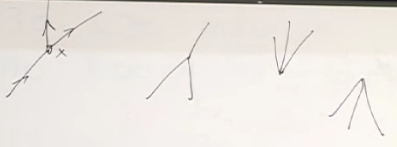
\includegraphics[width=0.8\textwidth]{phi-3-x}
\end{figure}

Figure \ref{fig:particles:fields:forces} shows a triangle of concepts. We have discussed two legs, Particles and Fields, but not the third, Forces.
\begin{itemize}
	\item Particles (\gls{gls:quanta} of fundamental fields)\footnote{We are going to have to think very hard about what is an elementary particle and what is composite; we will always be frustrated, always find some slippery reason why our definition did not work.}
	\item Fields
	\item Forces. 
\end{itemize}



\begin{figure}[H]
	\begin{center}
		\caption{Triangle of concepts: particles, fields, and forces}\label{fig:particles:fields:forces}
		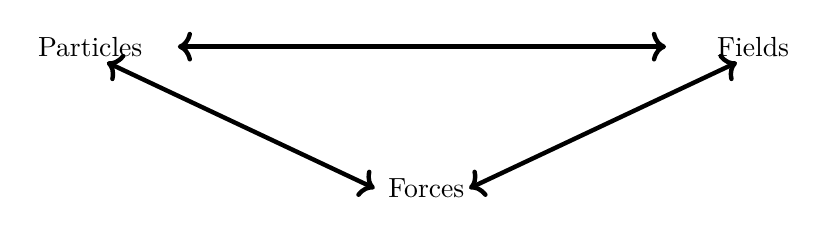
\begin{tikzpicture}	
			\filldraw[black] (-5, 2.0)  node[anchor=west]{Particles};
			\filldraw[black] (3.624, 2.0)  node[anchor=west]{Fields};
			\filldraw[black] (-0.55, 0.2)  node[anchor=west]{Forces};
			\draw[ultra thick, <->] (-3.1,2.0) --(3.1,2.0);
			\draw[ultra thick, <->] (-4.,1.8) --(-0.6,0.2);
			\draw[ultra thick, <->] (0.6,0.2) --(4.,1.8);
		\end{tikzpicture}
	\end{center}
\end{figure}

\subsection{Forces from Particles}

There must be a way of thinking about forces that depends on particles. We'll start by discussing it in classical electrodynamics. Suppose we put two electric charges into space, and we want to calculate the force between them. We could use Coulomb's law, or we could ask what they do to space--Figure \ref{fig:electric-field-due-to-first-charge}.

\begin{figure}[H]
	\begin{center}
		\caption{Electric Field due to first Charge}\label{fig:electric-field-due-to-first-charge}
		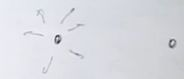
\includegraphics[width=0.8\textwidth]{electric-field-due-to-first-charge}
	\end{center}
\end{figure}

\begin{align*}
	E=&\int (e_1 \hat{E_1})^2 dV \text{, energy for first charge \emph{only}}
\end{align*}

\begin{itemize}
	\item The energy does not depend on the position of the charge.
	\item The energy contributes to the mass of the particle($E=mc^2$).
\end{itemize}

\begin{align*}
	E=&\int (e_1 \hat{E_1})^2 dV \text{, energy for second charge \emph{only}}
\end{align*}

Now we calculate the total energy.

\begin{align*}
	E=&\int (e_1\vec{E_1}+e_2 \vec{E_2})^2 dV\\
	=&\int \underbrace{(e_1\vec{E_1})^2}_\text{self energy}+ \underbrace{(e_2\vec{E_2})^2}_\text{self energy} + \underbrace{2e_1e_2\vec{E_1}.\vec{E_2}}_\text{interesting term}
\end{align*}

The first two terms represent self energy, which is included in mass; the last term is proportional to the charges.
\begin{itemize}
	\item  If they are so far away that $\vec{E_1}$ is negligible near second charge there will be no perceptible effect.
	\item If the particles are close we will get a contribution from $\vec{E_1}.\vec{E_2}$. This turns out to be the Coulomb force. 
\end{itemize}

The force comes from the distortion of the field: this is a \emph{purely field view of forces}. If fields give rise to forces, and particles are quanta of fields, there must be a way to think of forces coming from particles.

Where do molecular forces come from? There are several mechanisms: we will focus on one. Imagine two protons and a single electron--Figure \ref{fig:2protons:electron}. Electron hops because of tunnelling.

\begin{figure}[H]
	\begin{center}
			\caption[Molecular forces: two protons and a single electron]{Two protons and a single electron. Classically an electron can't swap between  (\subref{fig:2proton1Electrona}) and (\subref{fig:2proton1Electronb}), but \gls{gls:QM} allows it to tunnel. Don't attempt to watch tunnelling! It is like any \gls{gls:QM} effect; watching ruins it. You can wait on the left for electron to tunnel, but not on the right.}\label{fig:2protons:electron}
		\begin{subfigure}[t]{0.45\textwidth}
			\caption{Right hand proton is a long way from left. We show the Schr\"odinger wave function for electron near left hand.} 
			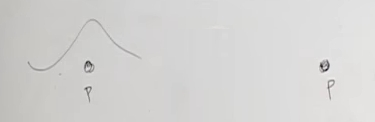
\includegraphics[width=0.9\textwidth]{2proton1Electrona}\label{fig:2proton1Electrona}
		\end{subfigure}
		\em
		\begin{subfigure}[t]{0.45\textwidth}
			\caption{Protons closer together: Figure \ref{fig:2proton1Electrona} still possible, but so is this; they have the same energy.}
			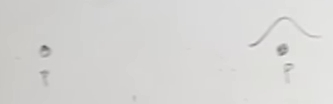
\includegraphics[width=0.9\textwidth]{2proton1Electronb}\label{fig:2proton1Electronb}
		\end{subfigure}
	\end{center}
\end{figure}

\begin{figure}[H]
	\begin{center}
		\caption[Effect of tunnelling]{Effect of tunnelling. It requires some energy to tunnel, which it gets back once it has tunneled. In the long term the electron spends an equal time on left or right, so it looks as if the two wave functions have been added, except it looks different in the middle.}
		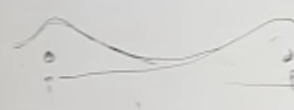
\includegraphics[width=0.9\textwidth]{2proton1Electronab}\label{fig:2proton1Electronab}
	\end{center}
\end{figure}

\begin{figure}[H]
	\caption{Energy as a function of distance between protons. Gradient in energy tries to move protons together, but Coulomb force tries to separate them; nett effect is a covalent bond.}
	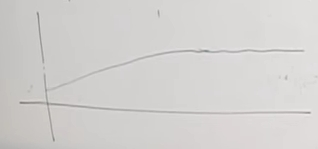
\includegraphics[width=0.9\textwidth]{2proton1ElectronEnergy}\label{fig:2proton1ElectronEnergy}
\end{figure}

\begin{figure}[H]
	\begin{center}
		\caption{Electron exchange between protons. This lowers energy relative to what it would be if there were only one proton and one electron. The presence of the electron between the two protons results in an attractive force. It is called particle exchange.}
		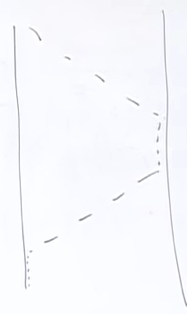
\includegraphics[width=0.5\textwidth]{2proton1ElectronHopping}\label{fig:2proton1ElectronHopping}
	\end{center}
\end{figure}

Energy is lowered by the possibility of alternating between two quantum states.

\begin{itemize}
	\item the electron being in a quantum superposition leads to a lower energy state, which creates a force;
	
	\item add 2nd electron, then total charge is zero, giving nett attraction; 

	\item so classically, add 2nd charge, lower energy (creates force) by distorting wave function;
	\item in \gls{gls:QM}, possibility of swapping between states lowers energy.
\end{itemize}
Can we think of Coulomb force in \gls{gls:QM} terms? Consider single proton and electron: proton interacts with electromagnetic field, whose quanta are photons.

\begin{itemize}
	\item Classically we solve field equations;
	\item In \gls{gls:QM} we think of emission and absorption of photons; this is what the Lagrangian tells us. One way to think of this is that the electron is a \gls{gls:QM} superposition of states:
	\begin{itemize}
		\item first of all states where there are no photons;
		\item a superposition of states in which a photon has been emitted;
		\item a superposition of states  with two photons emitted;
		\item photon reabsorbed, etc.
	\end{itemize}
	The net effect as a \gls{gls:QM} equilibrium of an electron surrounded by photons, which you can measure.
	 In Figure \ref{fig:2-1-electron-photons}, when electrons very far apart, energies just add. When they get closer, fields interact, or, in the language of Feynman diagrams, one electron absorbs electron emitted by the other--Figure \ref{fig:2-1-electron-photons-feynmann}.  Energy is no longer sum of energies of individual electrons, which gives rise to Coulomb force.
\end{itemize}

\begin{figure}[H]
	\caption{Emission and absorption of photons}
	\begin{subfigure}[t]{0.45\textwidth}
		\caption{Electron absorbing and reabsorbing photons.}
		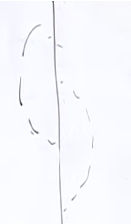
\includegraphics[width=0.9\textwidth]{2-1-electron-photons0}
	\end{subfigure}
	\begin{subfigure}[t]{0.45\textwidth}
		\caption{The electron is a \gls{gls:QM} superposition of states}\label{fig:2-1-electron-photons}
		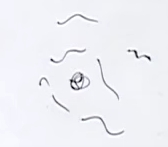
\includegraphics[width=0.9\textwidth]{2-1-electron-photons}
	\end{subfigure}

\end{figure}

\begin{figure}[H]
	\caption{Two Electrons }
	\begin{subfigure}[t]{0.45\textwidth}
		\caption{Two Electrons absorbing and reabsorbing photons.}\label{fig:2-1-second-electron-photons}
		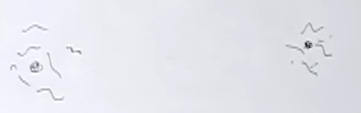
\includegraphics[width=0.9\textwidth]{2-1-second-electron-photons}
	\end{subfigure}
	\begin{subfigure}[t]{0.45\textwidth}
		\caption{Feynman diagram of Electrons absorbing and reabsorbing photons. Sometimes one electron absorbs photon emitted by other.}\label{fig:2-1-electron-photons-feynmann}
		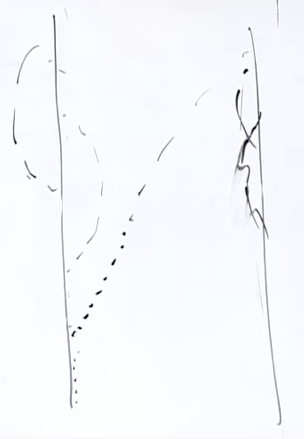
\includegraphics[width=0.9\textwidth]{2-1-second-electron-photons-feynman}
	\end{subfigure}
\end{figure}

In summary we have three ways of looking at forces:

\begin{itemize}
	\item laws such as Coulomb;
	\item classical field theory;
	\item exchange of particles. Every particle can be exchanged, so every particle produces a force: there are not just 4 forces! 
\end{itemize}

\subsection{Particles of the Standard Model}

The Standard Model is a mess. We don't understand why the particles are as they are. We understand some relationships, but there are more parameters, m More types of particles than known relationships.

\begin{table}[H]
	\begin{center}
		\caption{Some Particles and Fields}
		\begin{tabular}{|l|l|l|r|l|r|}\hline
			Name&Symbol&Statistics&Charge&B\#&Mass\\ \hline
			photon&$\gamma$ A&boson&0&0&0 \\ \hline
			electron&$e^\pm \Psi_e$&fermion&-1&0&$0.51\gls{gls:MeV}$\\ \hline
			quark&q(Q) $\Psi_q$&fermion&below&$\frac{1}{3}$&see below\\ \hline
			down&d&fermion&$-\frac{1}{3}$&$\frac{1}{3}$&10\gls{gls:MeV}\\ 
			up&u&fermion&$\frac{2}{3}$&$\frac{1}{3}$&5\gls{gls:MeV}\\ \hline
			strange&s&fermion&$-\frac{1}{3}$&$\frac{1}{3}$&100\gls{gls:MeV}\\ 
			charm&c&fermion&$\frac{2}{3}$&$\frac{1}{3}$&1\gls{gls:GeV}\\ \hline
			bottom&b&fermion&$-\frac{1}{3}$&$\frac{1}{3}$&5\gls{gls:GeV}\\ 
			top&t&fermion&$\frac{2}{3}$&$\frac{1}{3}$&170\gls{gls:GeV}\\ \hline
		\end{tabular}
	\end{center}
\end{table}

Notes:\begin{enumerate}
	\item Particle and Field usually have the same name, but there are a few exceptions, such as the vector potential $\boldsymbol{A}$.
	\item The electron has an electrical charge, so it must have an antiparticle. It is purely a matter of convention whether electron is particle and positron antiparticle, or vice versa. 
	\item Electric charge--electron is unit
	\item Mass--unit is electron Volt--eV
	\item $B\#$ denotes the Baryon number. Proton has Baryon number 1, antiproton -1, neutron +1, antineutron -1 (by convention). It isn't clear that baryon number is absolutely conserved: a proton may decay to something with zero baryon number, with a half life of $10^{33}$ years: this is an important question.
	\item Antiquarks have the charge and baryon number multiplied by -1.
	\item Mass of proton greatly exceeds mass of the 3 quarks.
	\item Mass of charmed quark exceeds mass of strange quark, reversing the behaviour of up and down. So different families have much the same behaviour, but widely different masses.
	\item Why are there 3 families of quarks? Nobody knows.
\end{enumerate}

\begin{figure}[H]
	\caption[The basic process in electrodynamics]{The basic process in electrodynamics is the emission of a photon by an electron. Out of this we can build all the processes of quantum electrodynamics, in particular the one that corresponds to the force between charges--see Figure \ref{fig:fep2}.}\label{fig:fep}
	\begin{subfigure}[t]{0.3\textwidth}
		\caption{Electron emits photon}
		\feynmandiagram[vertical = a to i1]{
			i1[particle=e]--[fermion]a--[fermion]o1[particle=e],
			a--[photon,edge label=$\gamma$]o2
		};
	\end{subfigure}
	\em
	\begin{subfigure}[t]{0.3\textwidth}
		\caption{Photon absorbed}
		\feynmandiagram[horizontal' = o2 to i1]{
			i1[particle=e]--[fermion]a--[fermion]o1[particle=e],
			a--[photon,edge label=$\gamma$]o2,
			o2--[draw=none]i1,
		};
	\end{subfigure}
	\em
	\begin{subfigure}[t]{0.3\textwidth}
		\caption{An electron traveling back in time is a positron}
		\feynmandiagram[vertical = a to o1]{
			i1[particle=e]--[fermion]a--[fermion]o1[particle=e],
			a--[photon,edge label=$\gamma$]o2
		};
	\end{subfigure}
	
\end{figure}


\begin{figure}[H]
	\begin{center}
		\caption{The processes of Figure \ref{fig:fep} visualized as exchange of a photon.}\label{fig:fep2}
		\feynmandiagram[vertical = i2 to i1]{
				i1 -- [fermion] a -- [fermion] i2,
				a -- [photon,edge label=$\gamma$] b,
				f1 -- [fermion] b -- [fermion] f2,
			};
	\end{center}
\end{figure}

Another way to describe Electromagnetic processes is to use a Lagrangian.
\begin{align*}
	\mathcal{L} =& \underbrace{e}_\text{Electric charge of electron} \underbrace{\Psi_e^\dagger}_\text{Create electron} \underbrace{\Psi_e}_\text{Annihilate electron} \underbrace{A}_\text{photon}
\end{align*}

The electric charge of electron is associated with the amplitude to emit a photon.


Three quarks build baryons; two quarks build mesons--Table \ref{table:mesons}.
\begin{itemize}
	\item neutron: $ddu$ (slightly heavier)
	\item proton: $uud$ (self energy of energy partially offsets difference in quark masses)
\end{itemize}

Can we make an analogue of proton/neutron with strange quarks? Yes. E.g. $sdu$, $ssu$, $uus$ -- Strange baryons.


\begin{table}[H]
	\begin{center}
		\caption[Mesons: baryon number 0 - quark + anti-quark]{Mesons: baryon number 0 - quark + anti-quark. Note the two entangled pairs: $\frac{1}{\sqrt{2}}\big(\ket{\bar{u}u}\pm\ket{\bar{d}d}\big)$}\label{table:mesons}
		\begin{tabular}{|l|l|l|r|} \hline
			&Quarks&Charge&Mass\\ \hline
			$\pi^-$&$\bar{u}d$&-1&$\approx140 \gls{gls:MeV}$ \\ \hline
			$\pi^+$&$u\bar{d}$&+1&$\approx140 \gls{gls:MeV}$  \\ \hline
			$\pi^0$&$\frac{1}{\sqrt{2}}\big(\ket{\bar{u}u}+\ket{\bar{d}d}\big)$&0&$\approx140 \gls{gls:MeV}$  \\ \hline
			$\eta$&$\frac{1}{\sqrt{2}}\big(\ket{\bar{u}u}-\ket{\bar{d}d}\big)$& 0&$\approx500 \gls{gls:MeV}$ \\ \hline
			$K^-$&$\bar{u}s$&-1& \\ \hline
			$K^+$&$u\bar{s}$&+1& \\ \hline
			$\bar{K}^0$&$\bar{d}s$&0& \\ \hline
			$K^0$&$d\bar{s}$&0& \\ \hline
			$\Phi$&$\bar{s}s$&0& \\ \hline
		\end{tabular}
	\end{center}
\end{table}

We also have strange mesons ($K-mesons$).


\section{Quantum Chromodynamics}\label{section:qcd}

This is the theory of quarks and gluons, and the things that they make.

\begin{defn}[Hadron]
	The things that quarks and gluons make are called hadrons. 
\end{defn}

There are 3 types of hadron: \begin{itemize}
	\item baryons, Definition \ref{defn:baryon};
	\item mesons, Definition \ref{defn:meson};
	\item glueballs, Definition \ref{defn:glueball}
\end{itemize}.

\begin{defn}[Baryon]\label{defn:baryon}
	An object made of 3 quarks is called a baryon: they always have spin $\frac{1}{2}$, $\frac{3}{2},...$.
\end{defn}

\begin{defn}[Meson][Baryon]\label{defn:meson}
	An object made of quark plus antiquark is called a meson; mesons are quark-anti-quark pairs.
\end{defn}

\begin{defn}[Gluon]
	Electrically neutral stuff than holds quarks and antiquarks together.
\end{defn}

\subsection{Spin without group theory}
We start with the basic commutation relations for angular momentum:\cite[Particle Physics 1]{susskind2007theoretical}
\begin{align*}
	[L_x,L_y] =& i \hslash L_z\\
	[L_y,L_z] =& i \hslash L_x\\
	[L_z,L_x] =& i \hslash L_y
\end{align*}

In a previous set of lectures,  we saw that:

\begin{itemize}
	\item we can break the symmetry by focusing on $L_z$
	\item we can measure only one $L_i$ at a time (they don't commute);
	\item $L_i$ is quantized--$\hslash$.
\end{itemize}

\begin{table}[H]
	\begin{center}
		\caption{Spin multiplets: Spin $l$ denotes highest $L_z$.}
		\begin{tabular}{|c|l|l|} \hline
		$l$&Range of $L_z (Number=2l+1)$&Statistics\\ \hline
		$0$&$0$& Boson\\ \hline
		$\frac{1}{2}$&$\{-\frac{1}{2},\frac{1}{2}\}$& Fermion\\ \hline
		$1$&$\{-1,0,1\}$&Boson \\ \hline
		$\frac{3}{2}$&$\{-\frac{3}{2},-\frac{1}{2},\frac{1}{2},\frac{3}{2}\}$&Fermion \\ \hline
		$2$&$\{-2,-1,0,1,2\}$&Boson \\ \hline
		\end{tabular}
	\end{center}
\end{table}

\begin{table}[H]
	\begin{center}
		\caption[Ways to put two spin $\frac{1}{2}$ particles together]{Ways to put two spin $\frac{1}{2}$ particles together. Consider whether particles could disappear with violating conservation of angular momentum. Notice the triplet and singlet.} 
		\begin{tabular}{|l|l|l|l|}\hline
			&$l$&$L_z$&Could disappear?\\ \hline
			$\ket{\uparrow\uparrow}$ &1&1&no: has $L_z$\\ \hline
			$\ket{\downarrow\downarrow}$&1&-1&no: has $L_z$ \\ \hline
			$\frac{1}{\sqrt{2}}(\ket{\uparrow\downarrow}+\ket{\downarrow\uparrow})$ &1&0&no: has $L_x$\\ \hline
			$\frac{1}{\sqrt{2}}(\ket{\uparrow\downarrow}-\ket{\downarrow\uparrow})$ &0&0&yes\\ \hline
		\end{tabular}
	\end{center}
\end{table}


\begin{table}[H]
	\begin{center}
		\caption{$3 \times \frac{3}{2}$ spins.}
		\begin{tabular}{|l|r|c|}\hline
			$\ket{\uparrow\uparrow\uparrow}$&$\frac{3}{2}$& \\ \hline
			$\ket{\downarrow\downarrow\downarrow}$&$-\frac{3}{2}$& \\ \hline
			$\ket{\uparrow\downarrow\downarrow}$,$\ket{\downarrow\uparrow\downarrow}$,$\ket{\downarrow\downarrow\uparrow}$&$\frac{1}{2}$&Three ways to do this\\ \hline
			$\ket{\uparrow\downarrow\downarrow}$,$\ket{\downarrow\uparrow\downarrow}$,$\ket{\downarrow\downarrow\uparrow}$&$-\frac{1}{2}$&Three ways to do this\\ \hline
		\end{tabular}
	\end{center}
\end{table}

\subsection{Isospin}

Isotopic spin was the first internal quantum number, the first analogue of spin, that did not have to do with the rotation of space. It had to do with the rotation of an internal space; it gave rise to a set of variables that were isomorphic to spin. You could imagine that it involves\d the rotation of some mathematical directions.

There is a whole variety of different kinds of quarks, but most of them are rather heavy, and had considerable mass in \gls{gls:GeV}, when the natural mass scale for hadrons is hundreds of \gls{gls:GeV}. The mass of a typical meson is 200 \gls{gls:MeV}, as it a typical binding energy for the quarks in a neutron; then binding energy of a nucleus is typically a few \gls{gls:MeV}. There are only two quarls whose mass is less, the up quark and the down quark. The others are heavy, and there is a cost in energy to make particles out of them. The most stable particles are the lightest, and they are the ones made out of up and down quarks.

The natural energy of the nucleus is a few hundred \gls{gls:MeV}, which comes from up and down quarks. To a first approximation masses are close to each other, so they are analogous to spin in some mathematical space. We have a symmetry. If we think of up and down quarks as isomorphic to up and down spins, we invent the concept of isotopic spin.

\begin{itemize}
	\item $(\uparrow,\downarrow)$ gives ordinary spin;
	\item $(u,d)$ Isotopic spin i.e.  $(p,n)$--makes Isotope.
\end{itemize}

Isotopic spin isn't a precise symmetry of nature, as $u$ and $d$ have different masses and charges. But it is an approximate symmetry for strong forces only. NB: for small nuclei, the strong force dominates electrostatic.

One quark is not an object that we can study in the laboratory: the simplest object we can study is 3 quarks. We can make an object of isotopic spin $\frac{1}{2}$ or $\frac{3}{2}$--Table \ref{table:3quark}.

\begin{itemize}
	\item Assume that we can label quarks--${1,2,3}$
	\item Quarks are Fermions, so we need to anti-symmetrize. For example the proton might be: $\underbrace{d_1}_\text{isospin $\frac{1}{2}$}\underbrace{(u_2u_3-u_3u_2)}_\text{isospin 0}$.
	\item $\frac{1}{2}$: two states (isotopic spin doublet--$p+n$)
	\item $\frac{3}{2}$. $uuu$ and $ddd$, $\uparrow\uparrow\uparrow$, $\downarrow\downarrow\downarrow$. There are 4 states for isospin $\frac{3}{2}$--an isospin multiplet. NB, this $\Delta_\frac{3}{2}$ differs from the nucleon, as all spins are aligned. The $uud$ and $uud$ have an isospin component of $\frac{1}{2}$, even though total isotopic spin is $\frac{3}{2}$.
\end{itemize}

\begin{table}[H]
	\begin{center}
		\caption[Simplest object we can study is 3 quarks.]{Simplest object we can study is 3 quarks. We can make an object of isotopic spin $\frac{1}{2}$ or $\frac{3}{2}$. Figure \ref{fig:decay:delta} shows the decay of $\Delta_\frac{3}{2}$.}\label{table:3quark}
		\begin{tabular}{|c|c|c|c|r|r|}\hline
			Isospin&Quarks&Spin&Name&Charge&Mass\\ \hline
			$\frac{1}{2}$&$duu$&$\frac{1}{2}$&proton&$+1$&940\gls{gls:MeV}\\ \hline
			$\frac{1}{2}$&$udd$&$\frac{1}{2}$&neutron&0&940\gls{gls:MeV}\\ \hline
			$\frac{3}{2}$&$uuu$&$\frac{3}{2}$&$\Delta_\frac{3}{2}$&$+2$&1200\gls{gls:MeV}\\ \hline
			$\frac{3}{2}$&$ddd$&$\frac{3}{2}$&$\Delta_\frac{3}{2}$&-1&1200\gls{gls:MeV}\\ \hline
			$\frac{3}{2}$&$uud$&$\frac{3}{2}$&$\Delta_\frac{3}{2}$&+1&1200\gls{gls:MeV}\\ \hline
			$\frac{3}{2}$&$udd$&$\frac{3}{2}$&$\Delta_\frac{3}{2}$&0&1200\gls{gls:MeV}\\ \hline
		\end{tabular}
	\end{center}
\end{table}

\begin{figure}[H]
	\begin{center}
		\caption[Decay of a $\Delta_\frac{3}{2}$]{Decay of a $\Delta_\frac{3}{2}$. Quarks can't go off on their own, so we need a quark-antiquark pair to balance. $\Delta_\frac{3}{2}\rightarrow p +\pi^+$: there is enough energy in $\Delta_\frac{3}{2}$ to create the $\pi^+$.}\label{fig:decay:delta}
		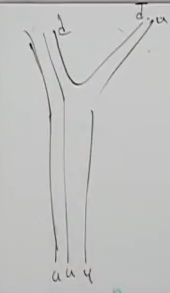
\includegraphics[width=0.5\textwidth]{2-2-Delta-decay}
	\end{center}
\end{figure}

\subsection{Quantum Chromodynamics}

We have a problem: $uuu$ represents three Fermions whose spins are all in the same direction, which violates the Pauli Exclusion Principle. Quarks must have another property, i.e. the three quarks must have a label which is hidden from view and not apparent in experiments. This is called \emph{colour}, a totally arbitrary name which has nothing to do with ordinary colour: it is just a name. Values are Red, Blue, and Green. The important thing is that they have precisely 3 different values.

Uhlenbeck and Goudsmit  \emph{might} have  discovered spin the same way, as helium has two electrons that are otherwise in the same state. Nambu Yoichiro realized that another quantum number was necessary for quarks.

The  $\Delta_\frac{3}{2}$ is important because of having 3 u or d. For proton we need to [anti?]symmetrize: $\ket{d_R u_G u_B}+...$

Note that for ordinary spin we need on particle to set a direction before we can say that a particular spin is down. One particle can set a frame of reference for the others.

What holds quarks together? Electrons use photons/electromagnetic field. Quarks use gluons: spin 1, so same polarization states, massless, but one big difference(later), and they jump back and forth. Quarks emit and absorb gluons.

The fundamental electromagnetic process is depicted in Figure \ref{fig:fep}. A photon is similar to electron and positron, e.g. it has the same properties: a sufficiently energetic photon can decay into an electron and positron pair.

\begin{figure}[H]
	\caption{Gluons}
	\begin{subfigure}[t]{0.45\textwidth}
		\caption{Introducing the gluon}\label{fig2-2-gluon1}
		\feynmandiagram[vertical = o1 to i1]{
			i1[particle=q]--[fermion]a--[fermion]o1[particle=q],
			a--[gluon]o2
		};
	\end{subfigure}
	\begin{subfigure}[t]{0.45\textwidth}
		\caption{A gluon behaves a bit like a quark-antiquark pair: this shows the gluon of Figure \ref{fig2-2-gluon1} as a fictitious quark-antiquark pair.  (Similarly you can think of a photon as a neutron-positron pair.)}
		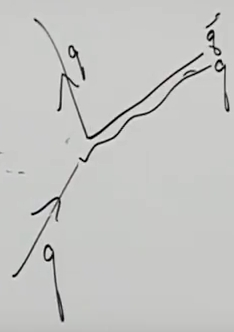
\includegraphics[width=0.9\textwidth]{2-2-gluon2}
	\end{subfigure}

\end{figure}

There appear to be 9 possible gluons: in Section \ref{sec:3:3:8} we will see that there are actually only 8, as the superposition $R\bar{R}+G\bar{G}+B\bar{B}$ is not an independent state.
\begin{align*}
\begin{pmatrix}
R\bar{R}&R\bar{G}&R\bar{B}\\
G\bar{R}&G\bar{G}&G\bar{B}\\
B\bar{R}&B\bar{G}&B\bar{B}
\end{pmatrix}
\end{align*}

Figures \ref{fig:2-2-gluon3} and \ref{fig:2-2-gluon5} show the basic vertices for gluons. Figures \ref{fig:2-2-gluon4} and \ref{fig:2-2-gluon6} redraw them, using a fictitious quark-antiquark pair. Gluons can interact with each other--Figure \ref{fig:2-2-gluon6}.
\begin{figure}[H]
	\caption{The basic vertices of \gls{gls:QCD} -- Quarks}
	\begin{subfigure}[t]{0.45\textwidth}
		\caption{Red quark changes to green: analogous to process with photon.}\label{fig:2-2-gluon3}
		\feynmandiagram[horizontal'= o1 to o2]{
			i[particle=\(R\)] -- [fermion]c,
			c -- [fermion] o1[particle=\(G\)],
			c -- [gluon]o2[particle=\(R\bar{G}\)],
		};
	\end{subfigure}
	\begin{subfigure}[t]{0.45\textwidth}
		\caption{Red quark changes to green, using fictitious quark-antiquark pair}
		\label{fig:2-2-gluon4}
		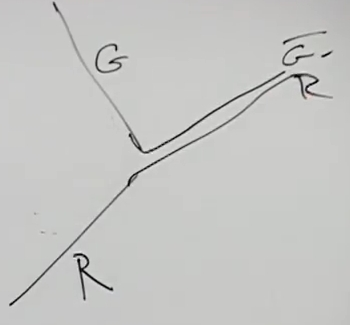
\includegraphics[width=0.9\textwidth]{2-2-gluon4}
	\end{subfigure}

\end{figure}

\begin{figure}[H]
	\caption{Second basic vertex of \gls{gls:QCD}: gluons}
		\begin{subfigure}[t]{0.40\textwidth}
		\caption{Second basic vertex, which has no analogue for photons. Fictitious quark-antiquark pairs represent gluons. This process makes \gls{gls:QCD} more complex and more interesting than QED.}\label{fig:2-2-gluon5}
		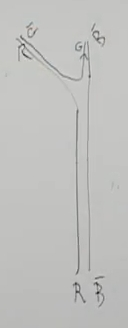
\includegraphics[width=0.9\textwidth]{2-2-gluon5}
	\end{subfigure}
	\em
	\begin{subfigure}[t]{0.45\textwidth}
		\caption{Second basic vertex, redrawn with gluons, instead of fictitious quark-antiquark pairs. Use Figure \ref{fig:2-2-gluon5} to determine which combinations don't break any lines.}\label{fig:2-2-gluon6}
		\feynmandiagram[horizontal'= o1 to o2]{
			i[particle=\(R\bar{B}\)] -- [gluon]c,
			c -- [gluon] o1[particle=\(R\bar{G}\)],
			c -- [gluon]o2[particle=\(G\bar{B}\)],
		};
	\end{subfigure}
\end{figure}

Photons cannot exchange photons, but gluons can exchange gluons, which means that there are \emph{forces between gluons}--Figure \ref{fig:quarks:gluons:forces}. Two waves of gluons can deform each other; different parts of one wave of gluons can deform each other, so the dynamics is non-linear.

\begin{figure}[H]
	\caption{Photons cannot exchange photons, but gluons can exchange gluons.}\label{fig:quarks:gluons:forces}
	\begin{subfigure}[t]{0.45\textwidth}
		\caption{Force between quarks}
		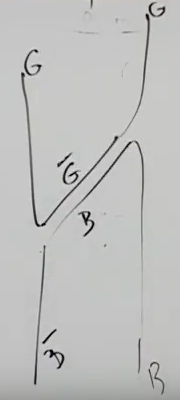
\includegraphics[width=0.9\textwidth]{2-2-gluon7}
	\end{subfigure}
		\begin{subfigure}[t]{0.45\textwidth}
		\caption{Force between gluons}
		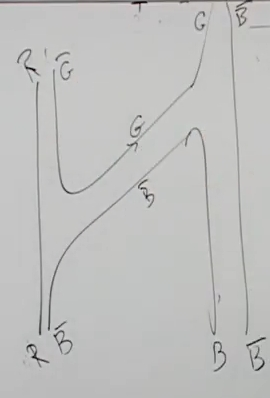
\includegraphics[width=0.9\textwidth]{2-2-gluon8}
	\end{subfigure}
\end{figure}

The only rule is: follow the lines and, if the line turn around, change particle to antiparticle.

Figure \ref{fig:2-2-mass1} shows that masses of objects are frequency dependent. In the same sense, masses of quarks depend on frequency.
\begin{itemize}
	\item  Move slowly and we drag gluons with quark.
	\item Move at high frequency, we drag the quark $m$ only
\end{itemize}

\begin{figure}[H]
	\caption[Mass (quark) with squishy thing attached]{Mass with squishy thing attached. If we move slowly we drag attachment, fast we just move mass. The concept of mass of quark is ambiguous: normally we mean the high frequency mass.}\label{fig:2-2-mass1}
	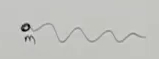
\includegraphics[width=0.8\textwidth]{2-2-mass1}
\end{figure}


\section{Group Theory I: Group Representations}

Rotations in space act on vectors: they rotate one vector to another. Rotations can be combined: they form a non-Abelian group. Figure \ref{fig:2-3-paramerize-rotation} depicts one way to parametrize rotation--axis $\vec{n}$ and angle $\theta$. Since $\vec{n}$ can be parametrized by two angles, latitude and longitude, we need 3 angles in total.

\begin{figure}[H]
	\begin{center}
		\caption{Parametrize rotation: axis $\vec{n}$ and angle $\theta$}\label{fig:2-3-paramerize-rotation}
		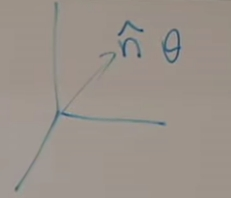
\includegraphics[width=0.8\textwidth]{2-3-paramerize-rotation}
	\end{center}
\end{figure}

Colour is a representation of the rotation group.

How do we construct a matrix representation of rotations? 

\begin{align*}
	R \vec{V} =&\vec{V^\prime} \text{, or, using indices}\\
	\sum_j R_{ij}(\theta,\vec{n})V_j=&V_i^\prime  \text{. Now if $R$ is a rotation, it doesn't change length}\\
	\forall \vec{V} \; \sum_i V_i^2 =& \sum_i (V_i^\prime)^2\\
	\sum_{i,j,k} R_{ij} R_{ik} V_j V_k =& \sum_i V_i V_i \text{, i.e.}\\
	\sum_{i} R_{ij} R_{ik} =& \delta_{j,k} \text{, or}\\
	R^T R =& I
\end{align*}

There are 3D representations of the rotation group. Can we think of them being related to quantum states? Spin describes angular momentum. A spin 1 particle (vector boson) can be described by a column vector containing amplitudes for the various components of spin. What about spin $\frac{1}{2}$ particle?

\begin{align*}
	\begin{pmatrix}
		1\\
		0
	\end{pmatrix}=& \ket{u}\\
	\begin{pmatrix}
		0\\
		1
	\end{pmatrix}=& \ket{d}\\
	\begin{pmatrix}
		\alpha_1\\
		\alpha_2
	\end{pmatrix}=& \alpha_1 \ket{u} + \alpha_2 \ket{v} \text{, where $\alpha_1^2+\alpha_2^2=1$}
\end{align*}

We can represent rotation by a $2\times2$ matrix acting on spinors.

\begin{align*}
	\begin{pmatrix}
		U_{11}&U_{12}\\
		U_{21}&U_{22}
	\end{pmatrix} 	\begin{pmatrix}
		\alpha_1\\
		\alpha_2
	\end{pmatrix} =& \begin{pmatrix}
		\alpha^\prime_1\\
		\alpha^\prime_2
	\end{pmatrix} \text{{. Now if}}\\
	\alpha^*_1 \alpha_1 + \alpha^*_2 \alpha_2 =& 1 \text{ we want}\\
	(\alpha^\prime_1)^* (\alpha^\prime_1) + (\alpha^\prime_2)^* (\alpha^\prime_2) =& 1 \text{, which gives}\\
	(U^T)^* U =& I \text{, which can be written} \\
	U^\dagger U =& I \numberthis \label{eq:unitary:2}
\end{align*}


$U$ has 8 degrees of freedom, but (\ref{eq:unitary:2}) imposes 4 constraints, leaving 4 degrees of freedom. But 3D rotations only have 3 degrees of freedom. We set $\det(U)=1$ to give a 2 parameter group, $SU(2)$

\begin{defn}[Unitary group $U(N)$]
	The group of unitary $N\times N$ matrices.
\end{defn}

\begin{defn}[Special Unitary group $SU(N)$]
	The subgroup of $U(N)$ with determinant 1.
\end{defn}

\begin{thm}[Infinitesimal generators of $SU(N)$]
	Any small rotation in $SU(N)$ can be expressed as:
	\begin{align*}
		U =& I + i \epsilon M \text{, where $M$ is a linear combination of the Pauli matrices $\sigma_i$}\\
		\sigma_x =& \begin{pmatrix} \numberthis \label{eq:pauli:x}
		0&1\\
		1&0
		\end{pmatrix}\\
		\sigma_y =& \begin{pmatrix} \numberthis \label{eq:pauli:y}
		0&-i\\
		i&0
		\end{pmatrix}\\
		\sigma_z =& \begin{pmatrix} \numberthis \label{eq:pauli:z}
		1&0\\
		0&-1
		\end{pmatrix}
	\end{align*}
\end{thm}

\begin{proof}
	We need two results, Lemmas \ref{lemma:det:Tr} and \ref{lemma:traceless:22}.
	\begin{lemma}[Determinant and Trace]\label{lemma:det:Tr}
		\begin{align*}
		\det( I + i \epsilon M) =& 1 + i\epsilon Tr(M) + O(\epsilon^2)
		\end{align*}
	\end{lemma}
	\begin{proof}
		We will prove by induction on $N$.
		
		
		\emph{Case: $N=1$.}
		\begin{align*}
			M =&\begin{bmatrix}
				M_{11}
			\end{bmatrix}\\
			\det( I + i \epsilon M) =& \det(\begin{bmatrix}
				1 + i \epsilon M_{11}
			\end{bmatrix}
			)\\
			=& 1 + i \epsilon M_{11}\\
			=&  1 + i\epsilon Tr(M)
		\end{align*}
		\emph{Case: $N>1$ and the Lemma is true for $N-1$}. We can find a (N-1)\times(N-1)matrix $M^{\prime}$, and two vectors $O(\epsilon)$ such that:
		\begin{align*}
			M =& \begin{bmatrix}
				1 + i \epsilon M_{11}&O(\epsilon)\\
				O(\epsilon)&M^{\prime} 
			\end{bmatrix}
		\end{align*}
		We will calculate the determinant by multiplying each element in the first row by its cofactor, then adding these terms. The first term is $(1 + i \epsilon M_{11})\det(M^{\prime})$. The other terms are products of $O(\epsilon)$ and a cofactor which includes a column of $O(\epsilon)$, so they are $O(\epsilon^2)$. Whence:
		\begin{align*}
			\det( I + i \epsilon M) =& 	(1 + i \epsilon M_{11}) \det(M^{\prime})+ O(\epsilon^2)\\ 
			=& \big(1 + i \epsilon M_{11}\big)\big(1 + i\epsilon Tr(M^{\prime}) + O(\epsilon^2)\big) + O(\epsilon^2)\\
			=& 1 + i \epsilon M_{11} + i\epsilon Tr(M^{\prime}) + O(\epsilon^2)\\
			=&1 + i\epsilon Tr(M) + O(\epsilon^2)
		\end{align*}
	\end{proof}
	
	\begin{lemma}[Traceless Hermitian $2\times2$ matrix]\label{lemma:traceless:22}
		Any traceless Hermitian $2\times2$ matrix can be written as a linear combination of the Pauli  matrices.
	\end{lemma}
	\begin{proof}
		The most general traceless Hermitian  $2\times2$ matrix can be written
		\begin{align*}
			\begin{pmatrix} 
				\alpha&\beta - i\gamma\\
				\beta + i\gamma&-\alpha
			\end{pmatrix} \text{, for some $\alpha$ and some real $\beta$ and $\gamma$.}
		\end{align*}
		\begin{align*}
			\begin{pmatrix} 
				\alpha&\beta - i\gamma\\
				\beta + i\gamma&-\alpha
			\end{pmatrix} =& \alpha  \begin{pmatrix} 
			1&0\\
			0&-1
			\end{pmatrix} +  \beta \begin{pmatrix} 
			0&1\\
			1&0
			\end{pmatrix} +  \gamma \begin{pmatrix} 
			0&-i\\
			i&0
			\end{pmatrix}\\
			=& \alpha \sigma_z + \beta \sigma_z + \gamma \sigma_y
		\end{align*}
		
	\end{proof}

	For small rotations:
	\begin{align*}
	\exists& M \text{ such that}\\
	U =& I + i \epsilon M \text{. Now}\\
	I =&U U^\dagger \text{ from (\ref{eq:unitary:2}), so}\\
	=& (I + i \epsilon M)(I - i\epsilon M^\dagger) \text{, which expands to}\\
	=& I + i \epsilon(M - M^\dagger) - \epsilon^2 M^\dagger \text{. If we discard $O(\epsilon^2)$}\\
	M - M^\dagger =& 0 \text{, i.e. M is Hermitean.}
	\end{align*}
	We also need U to be unimodular:
	\begin{align*}
	1=&\det(U)\\
	=& \det( I + i \epsilon M) \text{. Now, using Lemma \ref{lemma:det:Tr}}\\
	=& 1 + i\epsilon(Tr(M)) \text{, whence:}\\
	Tr(M) =&0
	\end{align*}
	
	So M satisfies the preconditions of Lemmas \ref{lemma:det:Tr} and \ref{lemma:traceless:22}, and the result follows immediately.
	
\end{proof}

State of quark can be Red, Green, or Blue. 
\begin{align*}
	\begin{pmatrix}
		\alpha_1\\
		\alpha_2\\
		\alpha_3
	\end{pmatrix} \leftrightarrow	\begin{pmatrix}
	\Psi_r\\
	\Psi_g\\
	\Psi_b
	\end{pmatrix}
\end{align*}

We can multiply by a member of $SU(3)$. These have $18-9-1=8$ degrees of freedom\footnote{$3\times 3$ matrix of complex numbers gives 18 real numbers; being unitary imposes 9 constraints; unimodularity adds one more}. Every term in Lagrangian needs to be invariant under $SU(3)$.  


\section{Group Theory – II}

\subsection{Group Theory}
$SU(2)$ is not exactly the same as 1D rotations: there is a $2\rightarrow1$ correspondence, not  $1\rightarrow1$, since $-U$ and $U$ correspond to the same rotation. This is why the electron wave function is called a doublet.

Generators are closely connected to infinitesimal elements. If you know the structure of the generators you can work out the whole structure of the group. Generators let us figure out conservation laws.

\begin{align*}
	U =& I + i \epsilon T\\
	I =& U^\dagger U + 1\\
	=& I + i\epsilon(T - T^\dagger) - \epsilon^2 T T^\dagger\\
	T =& T^\dagger \text{. Hermitian -- observable}\\
	\det(U) =& 1\\
	\implies&\\
	Tr(t)=&0
\end{align*}

Since the 3D rotation group has three parameters, the Ts span a 3D space. See (\ref{eq:pauli:x}), (\ref{eq:pauli:y}), and (\ref{eq:pauli:z}). We can figure out generators from commutation rules.

In SU(3) we have $3\times3$ matrices, so $3\times3\times2=18$ real components; the matrix being unitary imposes 9 constraints, and unimodularity imposes one more, whence there are $18-9-1=8$ degrees of freedom.

We can combine representations to form new representations. E.g. we might compose spins to make a composite. E.g. combine 2 spin $\frac{1}{2}$ objects. We have 4 possible states: a basis in that space can be thought of as a spin 0 object plus 3 spin 1 objects. We can make ${-1,0,+1}$, but the zero can be done in 2 ways: so one of the zero spins must not be part of the spin 1 multiplet, it can only be spin 0 (see ortho- and para-hydrogen).

\subsection{Representations of $SU(3)$.}

Triplet: $3\times3$ matrix acting on RGB vector, mixing up states, transforming to a quantum superposition.

There are 3 important representations: 

\subsubsection{The \bfseries{3}}

\begin{align*}
	\begin{pmatrix}
		q_r\\
		q_g\\
		q_b
	\end{pmatrix} \text{ field operator--creation}
\end{align*} 

\subsubsection{$\bar{3}$}

Antiquarks, represented by complex conjugates (not Hermitian conjugates)

\begin{align*}
	U q =& q^\prime\\
	U^* q^* = q^\prime& 
\end{align*}

Electron and positron are complex conjugate representations of $U(1)$. ($e^{i\theta}\psi_e \rightarrow e^{-i\theta}\psi_p$).

Generators of $\bm{\bar{3}}$ are negatives of generators of {\bfseries 3}, so they carry negative colour.

\subsubsection{$3 \otimes 3$}\label{sec:3:3:8}

Combine two quarks ${RR, RG, RB,...}$

\begin{align*}
	3 \otimes 3 =& \underbrace{\bar{3}}_\text{combine antisymmetrically} \oplus \underbrace{6}_\text{combine symmetrically}\\
	3 \otimes \bar{3} =& \underbrace{1}_\text{singlet: $R\bar{R}+G\bar{G}+B\bar{B}$} \oplus \underbrace{8}_\text{8 dimensional representation--generators!}
\end{align*}

\begin{align*}
3 \otimes 3 \otimes 3 =& (3 \otimes 3) \otimes 3\\
=& \big(\bar{3} \oplus 6 \big) \otimes 3\\
=& \bar{3}   \otimes 3 + 6 \otimes 3\\
=& \underbrace{1}_\text{anti-symmetrized superposed R, G, B} \oplus 8 \oplus 8 \oplus 10
\end{align*}

Gluon behaves a quark-antiquark under colour symmetry: it transforms under the 8 (octet).

\subsection{Quantum Chromodynamics (resumed)}

\begin{table}[H]
	\begin{center}
		\caption{Postulates of \gls{gls:QCD}.}\label{table:postulates:QCD}
		\begin{tabular}{|l|c|p{8cm}|} \hline
			Particle&Group&Remarks \\ \hline
			Quark&{\bfseries 3}& \\ \hline
			Antiquark&$\bm{\bar{3}}$& \\ \hline
			gluon&{\bfseries 8}&$\bm{3}\otimes\bm{3}=\bm{8}\oplus\bm{1}$, but the $\bm{1}$ does not exist in nature. It also doesn't mix with other components, so it is consistent to throw it away \\ \hline
			Free particles&{\bfseries 1}&All observable particles transform as singlets: quark+antiquark, or 3 quarks.\\ \hline
			&&Gluons play the same role in QCD as photons in QED, sourced from the 8 generators--Figure \ref{fig:2-4-quark-gluon-field}. Just as electric field of two particles has lower energy if total charge zero, gluon fields have lowest energy if total colour zero. But coupling constant higher, which is why we don't see free quarks.\\ \hline
		\end{tabular}
	\end{center}
\end{table}

What if we combine gluons together, or gluons with quarks?

\begin{defn}[Glueball][Baryon]\label{defn:glueball}
	Combine two gluons. $\bm{8} \otimes \bm{8} = \bm{63} \oplus \bm{1}$ -- 2 gluons. The singlet is known as a glueball.
\end{defn}

There are 3 kinds of Hadrons:
\begin{itemize}
	\item Baryons
	\item Mesons
	\item Glueballs
\end{itemize}

$SU(3)$ singlets also give integer charge, as phases cancel.

Back to $SU(2)$. We have $\Psi_i$. To make two particles act twice: $\Psi_i\Psi_j$, or $\Psi_i\Phi_j$(two different particles). We have a tensor-like object, having repeated indices.

\begin{align*}
	\begin{pmatrix}
		.&.&.&.\\
		.&.&.&.\\
		.&.&.&.\\
		.&.&.&.
	\end{pmatrix} 	\begin{pmatrix}
\Psi_u\Phi_u\\
\Psi_u\Phi_d\\
\Psi_d\Phi_u\\
\Psi_d\Phi_d
\end{pmatrix} 
\end{align*}
 The operator mixes things up, but we find
\begin{align*}
    \Psi_u\Phi_d-\Psi_d\Phi_u \text{, unchanged --singlet}	
\end{align*}
The next 3 mix among themselves and behave like a spin 1 object, the {\bfseries 3}.
\begin{align*}
	\begin{cases}
		\Psi_u\Phi_d+\Psi_d\Phi_u\\
		\Psi_u\Phi_u\\
		\Psi_d\Phi_d
	\end{cases}
\end{align*}

In the right basis:
\begin{align*}
	\begin{pmatrix}
		1&0&0&0\\
		0&.&.&.\\
		0&.&.&.\\
		0&.&.&.
	\end{pmatrix}
\end{align*}



The 8 gluons aren't neutral, as they have colour. The carry large amounts of energy, and don't appear as free particles. Gluons can interfere with each other, which is why QCD is more complicated than QED--see Figure \ref{fig:QCD:QED}.
 
\begin{figure}[H]
	\caption{Why QCD is more complicated than QED}\label{fig:QCD:QED}
	\begin{subfigure}[t]{0.45\textwidth}
		\caption[Quark surrounded by Gluon Field]{Quark surrounded by Gluon Field: there are 8 such fields, which transform according to the {\bfseries 8}.}\label{fig:2-4-quark-gluon-field}
		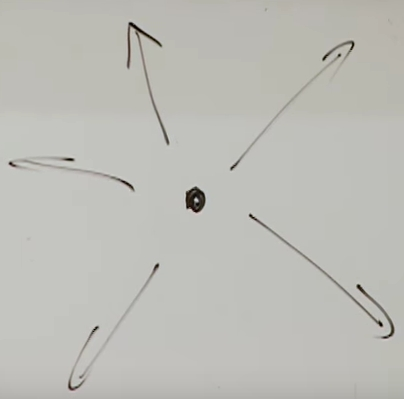
\includegraphics[width=0.9\textwidth]{2-4-quark-gluon-field}
	\end{subfigure}
	\begin{subfigure}[t]{0.45\textwidth}
		\caption{If Figure \ref{fig:2-4-quark-gluon-field} were an electromagnetic field, field lines would not attract or repel each other. In QCD they have colour, so they attract each other and form tubes.}
		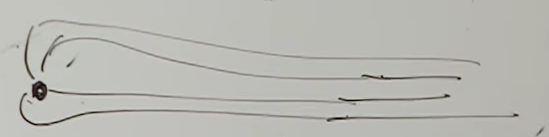
\includegraphics[width=0.9\textwidth]{2-4-quark-gluon-field-tubes}
	\end{subfigure}
	\begin{subfigure}[t]{0.45\textwidth}
		\caption{Tube linking quark and anti-quark-fluxoid. There is a uniform field, no matter how far particles separated.}
		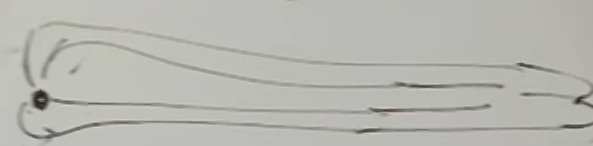
\includegraphics[width=0.9\textwidth]{2-4-quark-gluon-field-tubes-QAQ}
	\end{subfigure}
	\begin{subfigure}[t]{0.45\textwidth}
		\caption{Fluxoid. There is a uniform energy per unit length, so force increases as tube stretches. Unless flux tube ends at a quark/antiquark, energy is infinite.}
		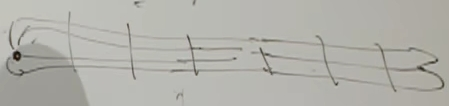
\includegraphics[width=0.9\textwidth]{2-4-quark-gluon-field-tube-uniform-energy}
	\end{subfigure}
	\begin{subfigure}[t]{0.45\textwidth}
		\caption{If meson has enough energy, tube may break, using quark-antiquark pair from vacuum. This forms a jet.}
		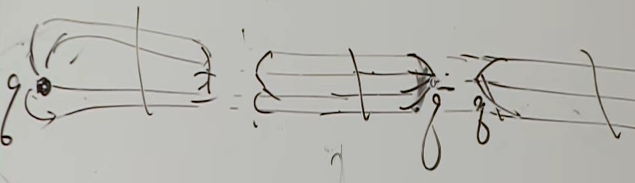
\includegraphics[width=0.9\textwidth]{2-4-split-meson}
	\end{subfigure}
\end{figure}

QCD is a gauge field--Sections \ref{section:gauge:symmetry} and \ref{section:gauge:invariance}.

\begin{defn}[Gauge field]\label{defn:gauge:field}
	A gauge field is any theory where conserved quantities are coupled to a Maxwell-like field. They are always based on symmetries.
\end{defn}

Charges linked are linked by lines of force. In Figure \ref{fig:2-4-quark-gluon-field}, fields lines must end on charge means charge conserved, which related to symmetry.

\section{Gauge Fields and Symmetry}\label{section:gauge:symmetry}

\subsection{Gauge Fields and Symmetry}

Just about all of nature is controlled by gauge theories.

The first and simplest gauge theory is Maxwell's theory. This has six components, the electric and magnetic fields, which are generated from a potential $A_\mu=(A_0,\vec{A})$.
\begin{itemize}
	\item  $A_0$ is the electric potential: $F_i=e \frac{\partial A_0}{\partial x_i}$.
	\item Electric field $\vec{E}=\nabla A_0$.
	\item Magnetic field $\vec{B}=\nabla \times \vec{A}$
\end{itemize}

The electric and magnetic fields combine to make the field tensor\cite{susskind2017special}:
\begin{align*}
	F_{\mu,\nu} =&\begin{pmatrix} \numberthis \label{eq:field:tensor}
		0&-E_x&-E_y&-E_z\\
		E_x&0&B_z&-B_y\\
		E_y&-B_z&0&B_x\\
		E_z&B_y&-B_x&0
	\end{pmatrix}
\end{align*}

\begin{figure}[H]
	\caption[Electromagnetic waves, illustrating Polarization.]{Electromagnetic waves. Polarization is in direction of electric field.}
	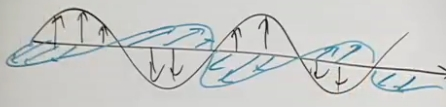
\includegraphics[width=0.8\textwidth]{2-5-EM-field}
\end{figure}

The essence of a gauge theory: in Maxwell-like theories, with electric-like and magnetic-like fields, if gauge field is weakly coupled (interactions between parts don't interfere with each other), motion of a gauge field is exactly the same as a light wave; it moves at the speed of light unless something interferes.

Gauge theories  always have conserved quantities, hence symmetries. Colour is an example.
\begin{itemize}
	\item  Let $A_{ij}$ denote the potential, which transforms under $SU(3)$.
	\item Symmetry: $U_{ij} q_j = q^\prime_i$ (indexed over colour).
	\item The $q_i$ form a representation of $SU(3)$, known as the fundamental representation.
	\item The antiparticles are represented $U^*_{ij} q^*_j = q_i^{\prime*}$. We have two distinct representations, {\bfseries 3} and $\bm{\bar{3}}$.
	\item  $A_{ij}$ has same structure as $\bar{q}_i q_j$.
	\item $A_{ij}$ transforms like quark/antiquark, and  trace vanished (adjoint representation).
	\item $A_{ij}$ transforms according to $SU(3)$  (unlike photon--not charge).
\end{itemize}

\begin{figure}[H]
	\caption{Basic interactions of gauge theory}
	\begin{subfigure}[t]{0.45\textwidth}
		\caption{i becomes j by emitting a quantum of field $A_{ji}$}
		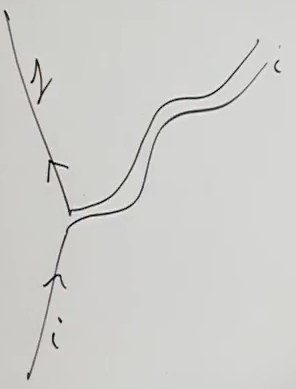
\includegraphics[width=0.9\textwidth]{2-change-charge} 
	\end{subfigure}
	\begin{subfigure}[t]{0.45\textwidth}
		\caption{Interaction with gluons only: they exert forces that photons don't.}
		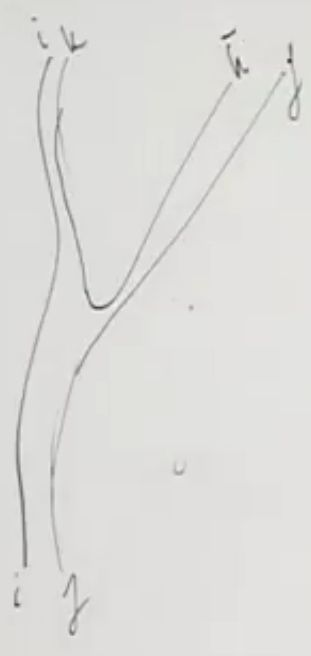
\includegraphics[width=0.9\textwidth]{2-5-gluon-gluon}
	\end{subfigure}
\end{figure}

\subsection{Strong and Weak Interactions}

A Gauge theory also needs a coupling constant, analogous to the charge of the electron (amplitude for emitting photon). EM is weak: probability of emission is $\frac{1}{137}$.

Set $c=1$, $\hslash=1$, then energy is in units of $\frac{1}{T}$: $1eV^{-1}=10^{-7}M$.

\subsubsection{Strong and Electromagnetic Interactions}

Table \ref{table:ems} compares various properties of the Strong and Electromagnetic Interactions.

\begin{table}[H]
	\begin{center}
		\caption{Electromagnetic and strong}\label{table:ems}
		\begin{tabular}{|l|r|r|} \hline
			&Atom&Hadron \\ \hline
			$\alpha$&$\frac{1}{137}$&\\ \hline	
			Diameter atom&$10^{-10}M$&$10^{-15}M$ \\ \hline
			Transit time &$10^{-18}S$&$10^{-23}S$\\ \hline
			Orbital time &$10^{-18}S$&$10^{-23}S$\\ \hline
			Decay time (from $1^{st}$ excited state)&$10^{-9}S$&$10^{-23}S$\\ \hline
		\end{tabular}
	\end{center}
\end{table}

Times for Hadrons less spread out: QCD version of $\alpha$ much closer to 1 ($\frac{1}{5}$). This is why strong interactions are called \emph{strong}.

\subsubsection{Weak Interactions}

There is another set of interactions that are characterized by being quite slow. Table \ref{table:ex:weak} gives examples.

\begin{table}[H]
	\begin{center}
		\caption{Examples of Weak decay}\label{table:ex:weak}
		\begin{tabular}{|l|l|p{6cm}|}\hline
			$n \rightarrow e + p +\bar{\nu}$&12 minutes&Barely enough energy: 940\gls{gls:MeV} $\rightarrow$ 939\gls{gls:MeV} + 0.5\gls{gls:MeV}, but this isn't enough to explain the slowness.\\ \hline
			$\pi^- \rightarrow e^- + \bar{\nu} $&$10nS$&Plenty of energy, but still slow.\\ \hline
			$\pi^+ \rightarrow e^+ + \nu $&&\\ \hline
		\end{tabular}
	\end{center}
\end{table}

These are very slow: clearly something else is going on! Table \ref{tab:QCD:rows} is relevant. \begin{itemize}
	\item Colour symmetry, $SU(3)$, operates on rows; a $u$ remains a $u.$
	\item We introduce a new gauge symmetry, $SU(2)$ operating horizontally: $u\leftrightarrow d$;  $c\leftrightarrow s$;  $t\leftrightarrow b$.
\end{itemize}

\begin{table}[H]
	\begin{center}
		\caption{Quarks: Colour symmetry operates on first three rows, not on columns}\label{tab:QCD:rows}
		\begin{tabular}{|c|c|c|c|} \hline
			&u d&c s&t b \\ \hline
			red&x x&x x&x x\\ \hline
			green&x x&x x&x x\\ \hline
			blue&x x&x x&x x\\ \hline
			leptons&$\nu_e$ e&$\nu_\mu$ $\mu$&$\nu_\tau$ $\tau$\\ \hline
		\end{tabular}
	\end{center}
\end{table}

The last row deals with Leptons. They appear in an order that depends on the charge difference: $u-d=\nu_e-e$
 
We postulate a gauge boson that which combines a particle and an antiparticle, and apply it to leptons, e.g, $e \bar{\nu_e}$. We call this gauge boson, $W$:

 \begin{itemize}
 	\item $e \bar{\nu_e}\leftrightarrow W^- \leftrightarrow d\bar{u}$
 	\item $e^+ \nu_e\leftrightarrow W^+ \leftrightarrow \bar{d}u$
 \end{itemize}

This is sometimes known as the flavour symmetry.

Imagine that W is like photons or gluons, so it behaves as shown in Figure \ref{fig:W:photon:fluon}.

\begin{figure}[H]
	\caption{W are like photons or gluons}\label{fig:W:photon:fluon}
	\begin{subfigure}[t]{0.45\textwidth}
		\caption{$e \rightarrow\nu + W^-$}\label{fig:2-5-W1}
		\feynmandiagram[vertical=o1 to i1]{
			i1[particle=$e$]--[fermion] a--[fermion] o1[particle=$\nu$],
			a--[charged boson,edge label=$W^-$]o2
		};
	\end{subfigure}
	\begin{subfigure}[t]{0.45\textwidth}
		\caption{$d \rightarrow u + W^-$}
		\feynmandiagram[vertical=o1 to i1]{
			i1[particle=$d$]--[fermion] a--[fermion] o1[particle=$u$],
			a--[charged boson,edge label=$W^-$]o2
		};
	\end{subfigure}
	\begin{subfigure}[t]{0.45\textwidth}
		\caption{$s \rightarrow c + W^-$}
		\feynmandiagram[vertical=o1 to i1]{
			i1[particle=$s$]--[fermion] a--[fermion] o1[particle=$c$],
			a--[charged boson,edge label=$W^-$]o2
	};
	\end{subfigure}
	\begin{subfigure}[t]{0.45\textwidth}
		\caption{$W^+$ and $W^-$ are antiparticles, so we can redraw \ref{fig:2-5-W1}}
		\feynmandiagram[vertical=o1 to i1]{
			i1[particle=$e$]--[fermion] a--[fermion] o1[particle=$\nu$],
			o2--[charged boson,edge label=$W^+$]a
		};
	\end{subfigure}
\end{figure}

\begin{figure}[H]
	\caption{Examples of W boson mediated decays}
	\begin{subfigure}[t]{0.30\textwidth}
		\caption{Pion decay (electron, muon, tau, and associated neutrino)}
		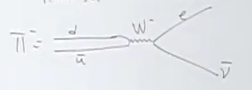
\includegraphics[width=0.9\textwidth]{2-5-pion-decay}
	\end{subfigure}
	\begin{subfigure}[t]{0.30\textwidth}
		\caption{Muon decay}
		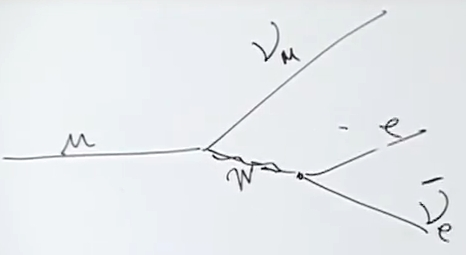
\includegraphics[width=0.9\textwidth]{2-5-muon-decay}
	\end{subfigure}
	\begin{subfigure}[t]{0.30\textwidth}
		\caption{Neutron decay. W doesn't have enough energy to make muon, unless we hit neutron really hard.}
		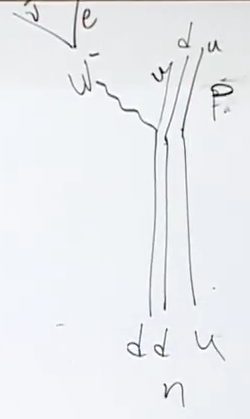
\includegraphics[width=0.9\textwidth]{2-5-neutron-decay}
	\end{subfigure}
\end{figure}

NB: can violate conservation of energy for a very short time(Heisenberg uncertainty).

Why so slow? Coupling constant?(No)

\section{The Weak Interaction}

\subsection{Why is the weak interaction so slow?}

In Table \ref{tab:QCD:rows} we have three symmetries: $SU(3) \otimes SU(2) \otimes U(1)$. We say that the Standard Model is a gauge theory based on  $SU(3) \otimes SU(2) \otimes U(1)$.

\begin{table}[H]
	\begin{center}
		\caption{Coupling Constants}
		\begin{tabular}{|l|l|l|} \hline
			Group&Coupling Constant&Remarks \\ \hline
			$U(1)$&e& \\ \hline
			$SU(3)$&$g_s \approxeq 1$& \\ \hline
			$SU(2)$&$g_w$& \\ \hline
		\end{tabular}
	\end{center}
\end{table}



\begin{figure}[H]
	\caption{Possible fates of a W boson}
	\begin{subfigure}[t]{0.5\textwidth}
		\caption{Decay of a neutron. The $W$ line is the \emph{propagator}}\label{fig:2-6-W1}
		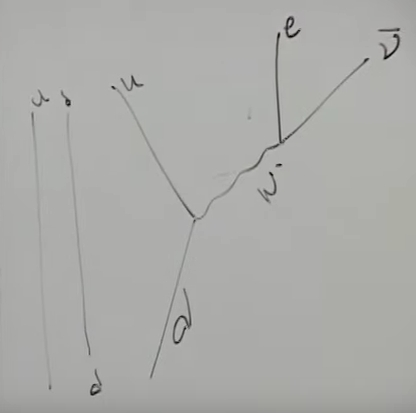
\includegraphics[width=\textwidth]{2-6-W1}
	\end{subfigure}
	\begin{subfigure}[t]{0.4\textwidth}
		\caption{A different fate for a W Boson: re-absorption}\label{fig:absorption:W:boson}
		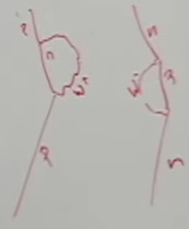
\includegraphics[width=\textwidth]{2-6-W2}
	\end{subfigure}
\end{figure}

The Propagator is a function of proper time between two points: $\Delta(ds)$. Figure \ref{fig:2-6-propagator} shows the dependence. For small distance $\Delta(ds)$ is independent of mass, but the values differ  after a certain distance: $\Delta(ds)$ falls sharply to zero.

\begin{figure}[H]
	\caption[Propagator $\Delta(ds)$ as a function of distance.]{Propagator $\Delta(ds)$ as a function of distance. Black line is for zero mass, $\frac{1}{ds}$, red for non-zero.}\label{fig:2-6-propagator}
	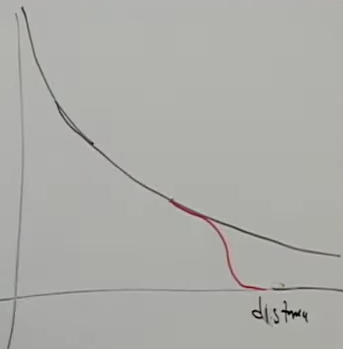
\includegraphics[width=0.8\textwidth]{2-6-propagator}
\end{figure}

Where does $\Delta$ decrease suddenly? Choose units where $c=\hslash=1$:
\begin{align*}
	[m] =& [E]\\
	=& [L^{-1}]\\
	=& [P]\\
	distance \propto & \frac{1}{L} \text{, in fact:}\\
	distance \approxeq & \frac{\hslash}{mc} \text {, Compton wavelength}
\end{align*}

$\Delta^2(ds)$ is the probability particle can get that far.

In an experiment, we know the momenta. We can think of propagator as function of position, or momentum--using Fourier transform:
\begin{align*}
\tilde{\Delta}(k_w)=\frac{1}{k_w^2+m_w^2} \numberthis \label{eq:Delta}
\end{align*}
 $\tilde{\Delta}(k_w)$ will have its biggest value when $k_w=0$, so the most likely thing is to emit a low momentum W, which costs an amplitude of $\frac{1}{m_w^2}$. Amplitude for emitting $W$ and converting to electron plus neutrino is $\frac{g_w^2}{m_w^2}$: weak interactions are made weak because the mass of the W is large--about 100 protons! Probability is $\frac{g_w^4}{m_w^4}$.
 
 W is a virtual particle. From the energy-time uncertainty principle, energy conservation can be violated briefly: $\delta T \delta E<\hslash$. There is not enough energy in neutron to make a real W, but it can briefly make a virtual W, which must be destroyed again.\footnote{I have left out a discussion where Prof Susskind shows that trying to watch the virtual particle is doomed to failure: briefly the photon we send in to observe the phenomenon, need very high energy, as the phenomenon is very short lived; the high energy photon upsets the apple-cart.}
 
 We can verify (\ref{eq:Delta}) by creating high momentum particles in an accelerator.
 
 Figure \ref{fig:absorption:W:boson} shows a different fate for a W-boson: re-absorption.
 
 Figure \ref{fig:2-6-photons} shows a process where photons \emph{can} interact, via the creation of a virtual pair. Since probability is proportional to the inverse of the energy required, we don't see it in the lab. Same thing happens with W bosons.
 
 \begin{figure}[H]
 	\caption[Photon interaction via the creation of a virtual pair]{Process where photons \emph{can} interact, via the creation of a virtual pair}\label{fig:2-6-photons}
 	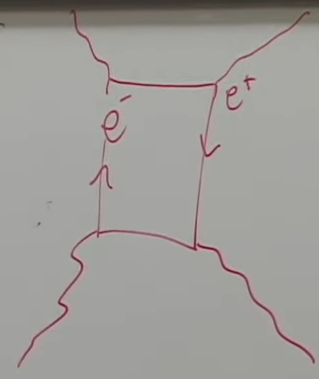
\includegraphics[width=0.8\textwidth]{2-6-photons}
 \end{figure}

The up quark and down quark go into each other by emitting a W. What group are we talking about? SU(2). But SU(2) has 3 generators; we are missing a gauge boson, $Z$. [Check that this is discussed in a later lecture.]

\subsection{Spontaneous symmetry breaking}
 
 One example is a bunch of spins that can either be up or down, e.g. classical coins, with an interaction so that energy is less if spins parallel. There are two states of lowest energy, both ground states. Figure \ref{fig:2-6-sponteneous} shows how one spin can break symmetry. This is not the same as explicit symmetry breaking--having a bias, where H has different energy from T.
 
 Spontaneous symmetry breaking is deficient from explicit symmetry breaking, as the former can introduce domain walls.
 \begin{figure}[H]
 	\begin{center}
 		\caption[Spontaneous symmetry breaking]{We have one coin, a long way from the other, in known state. This introduces a slight difference between two aligned states: it becomes expensive to add a Tail.}\label{fig:2-6-sponteneous}
 		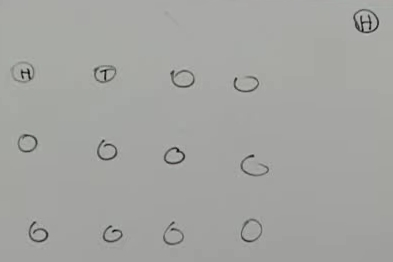
\includegraphics[width=0.8\textwidth]{2-6-sponteneous}
 	\end{center}
 \end{figure}

Spontaneous symmetry breaking has an instability that can let the system go one way or another.

\section{Spontaneous symmetry breaking and Goldstone bosons}

Our goal is to show how a particle like a photon can gain a mass from something called spontaneous symmetry breaking; how it can gain a mass from the Higgs mechanism. There are two important ingredients:

\begin{itemize}
	\item Spontaneous symmetry breaking
	\item gauge invariance.
\end{itemize}

\subsection{Spontaneous symmetry breaking}
In the last lecture we considered a system of spins that pointed up or down.
There is no fundamental asymmetry between up and down. Two up spins have the same energy as two downs; and an up and a down has the same energy as a down and an up. Because it is energetically favourable for them to be parallel, the spins should be all up or all down. The direction can be controlled by one spin very far away that is frozen. We have symmetry, but it is broken spontaneously; it may take a finite time to propagate.

Compare with explicit symmetry breaking, e.g. a magnetic field that is pointed up. Now energy will be lower for one direction.

What if we find aligned system, how do we know whether or not it is spontaneous? Domain walls: set one boundary to one direction, other to the other, and see what happens. If there is bias, then our change should not propagate in very far. If spontaneous we expect a domain wall to emerge.

We can imagine a real scalar field, $\Phi$, which behaves the same way. It has a Lagrangian:

\begin{align*}
	\mathcal{L} =& \frac{1}{2} \partial_\mu \Phi \partial^\mu \Phi - V(\Phi) \numberthis \label{eq:spontaneous:symmetry:L}
\end{align*}
where V has the form of Figure \ref{fig:2-7-V}.

Since $V$ is completely symmetric, there will be two ground states. Why can't system jump from $-f$ to $f$? A jump would make $\frac{\partial \Phi}{\partial x}$ very large. Figure \ref{fig:2-7-V-simple} shows a different potential, which does not lead to spontaneous symmetry breaking. Figure \ref{fig:2-7-V-domain-wall} shows how we can force a domain wall for Figure \ref{fig:2-7-V}, but not Figure \ref{fig:2-7-V-simple} (If temperature high there is lots of random fluctuation; domains appear when system cooled.).

\begin{figure}[H]
	\caption[$V(\Phi)$ with and without spontaneous symmetry breaking]{Potential for (\ref{eq:spontaneous:symmetry:L}), with and without spontaneous symmetry breaking}
	\begin{subfigure}[t]{0.45\textwidth}
		\vskip 0pt
		\caption{Possible spontaneous symmetry breaking: two ground states. This is not a continuous symmetry, as we can't interpolate between minima.}\label{fig:2-7-V}
		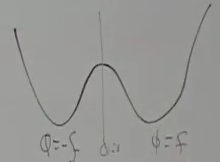
\includegraphics[width=0.8\textwidth]{2-7-V}
	\end{subfigure}
	\hfill
	\begin{subfigure}[t]{0.45\textwidth}
		\vskip 0pt
		\caption{Potential without spontaneous symmetry breaking: only one ground state}\label{fig:2-7-V-simple}
		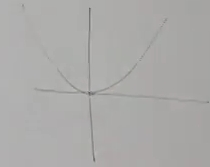
\includegraphics[width=0.8\textwidth]{2-7-V-simple}
	\end{subfigure}
	\hfill
	\begin{subfigure}[t]{0.9\textwidth}
		\begin{center}
			\caption{Domain wall for potential of Figure \ref{fig:2-7-V}}\label{fig:2-7-V-domain-wall}
			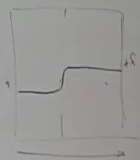
\includegraphics[width=0.8\textwidth]{2-7-V-domain-wall}
		\end{center}
	\end{subfigure}
\end{figure}

In both cases we have looked at breaking a discrete symmetry. What if we break a continuous symmetry, such as $U(1)$ or $SU(2)$? We will do one example of a continuous symmetry breaking, and the idea of a Goldstone boson (which replaces the idea of domain walls); we'll see how how the Goldstone boson can radically change its nature when the symmetry had to do with gauge bosons. It morphs from spontaneous symmetry breaking into the Higgs phenomenon. We will see how the Higgs mechanism allows the Z-boson to have mass.


Imagine a complex field, Figure \ref{fig:2-7-complex-phi}\footnote{The $\frac{1}{2}$ is normally omitted from $\mathcal{L}$ for complex fields.}.
\begin{align*}
	\Phi =& \Phi_R + i \Phi_I \\
	\Phi^* =& \Phi_R - i \Phi_I\\
	\mathcal{L} =&  \partial_\mu \Phi^* \partial^\mu \Phi 
\end{align*}

This is symmetric under U(1):
\begin{align*}
	\Phi \rightarrow \Phi^\prime=e^{i \theta} \Phi  \numberthis \label{eq:U1:theta}
\end{align*}

For the time being assume $\theta$ constant--but we will relax this in Section \ref{section:gauge:invariance}.

\begin{figure}[H]
	\caption{A complex field (not necessarily an analytic function)}\label{fig:2-7-complex-phi}
	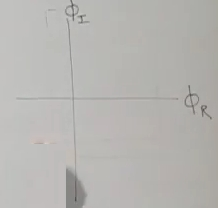
\includegraphics[width=0.8\textwidth]{2-7-complex-phi}
\end{figure}

Let's add a potential that shares this symmetry. We will focus on two kinds of potentials: one of them spontaneously breaks the symmetry, the other doesn't. We define a Lagrangian that is symmetrical about rotation in $\Phi$ plane:
\begin{align*}
\mathcal{L} =&  \partial_\mu \Phi^* \partial^\mu \Phi -V(\Phi \Phi^*) \text{, where}\\
V =& \Phi \Phi^* \text{, completely symmetric--\text{, see Figure \ref{fig:2-7-V-quad}}, or} \numberthis \label{eq:symmetric}\\
V=& -a \Phi \Phi^* + b (\Phi \Phi^*)^2 \text{, see Figure \ref{fig:2-7-V-quartic}} \text{, where $a>0,b>0$}\numberthis \label{eq:breakable:symmetric}
\end{align*}

\begin{itemize}
	\item At the origin, $\Phi \Phi^*$  is at a minimum. This is the ground state. There is no explicit or spontaneous breaking of symmetry.
	\item Near the origin, $-a \Phi \Phi^* + b (\Phi \Phi^*)^2$ is at a maximum. There are many ground states around the minimum circle. $\Phi$ wants to move away from zero, but not too far. It also doesn't want $\partial_\mu \Phi^* \partial^\mu \Phi$ to get too big, so we expect field to bunch \emph{somewhere} on minimum.
\end{itemize}

Are there domain walls? Figure \ref{fig:2-7-V-quartic-domain-wall} shows an attempt to check this. Note that we don't get an abrupt transition, as we need to keep $\partial_\mu \Phi^* \partial^\mu \Phi$ small.

\begin{figure}[H]
	\caption{Potentials}\label{fig:s-7-potentials}
	\begin{subfigure}[t]{0.5\textwidth}
		\caption{ $V=\Phi \Phi^*$-- Minimum at origin.}\label{fig:2-7-V-quad}
		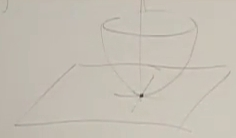
\includegraphics[width=\textwidth]{2-7-V-quad}
	\end{subfigure}
	\begin{subfigure}[t]{0.5\textwidth}
		\caption{$V=-a \Phi \Phi^* + b (\Phi \Phi^*)^2$--Minimum on circle of radius $f$.}\label{fig:2-7-V-quartic}
		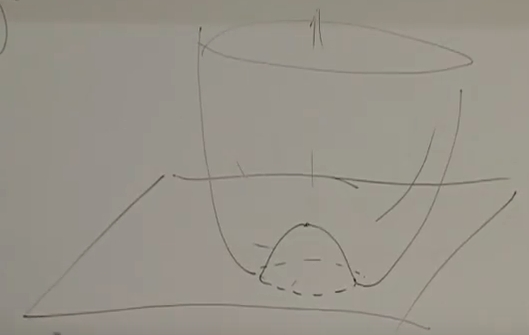
\includegraphics[width=\textwidth]{2-7-V-quartic}
	\end{subfigure}
	\begin{subfigure}[t]{0.5\textwidth}
		\caption{Clamp values to try to produce domain wall}\label{fig:2-7-V-quartic-domain-wall-ab}
		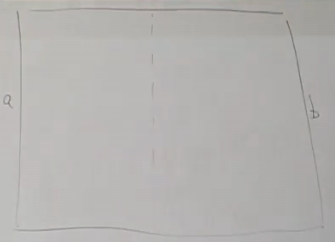
\includegraphics[width=\textwidth]{2-7-V-quartic-domain-wall-ab}
	\end{subfigure}
	\begin{subfigure}[t]{0.5\textwidth}
		\caption{We don't have the clamped values diametrically opposed to remove ambiguity.}\label{fig:2-7-V-quartic-domain-wall}
		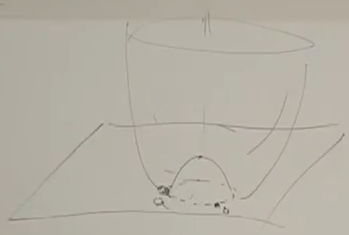
\includegraphics[width=\textwidth]{2-7-V-quartic-domain-wall}
	\end{subfigure}
\end{figure}

It turn out that the field varies smoothly between $a$ and $b$.

\begin{thm}[Mexican Hat Potential]
	Angle varies linearly
\end{thm}
\begin{proof}
	TBP -- use calculus of variations.
\end{proof}

 From the point of view of wave equations, a field with only gradient terms in energy is massless: quanta are massless. Also for field $e^{ikx}$, if $k=0$ makes energy $0$, then very long wavelength field has zero mass.
 
We will look at various potentials, starting with $\frac{m^2 \phi^2}{2}$--  Figure \ref{fig:2-7-V-simple}. It clear that if you created a wave that varied from place to place, no matter how long that wavelength was, as long as there is  variation away from zero, there is going to be an appreciable cost of energy--Figure \ref{fig:2-7-variation-from-zero}. This is a massive particle: if there is no mass, the only energy comes from gradient, and that is small for a long wavelength particle; $\frac{m^2 \phi^2}{2}$ is called a mass term.

\begin{figure}[H]
	\begin{center}
		\caption{There are a lot of places where wave away from zero, and those are going to cost energy.}\label{fig:2-7-variation-from-zero}
		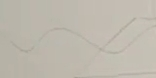
\includegraphics[width=0.6\textwidth]{2-7-variation-from-zero}
	\end{center}
\end{figure}

Returning to \ref{fig:2-7-V-quartic}, let's try to identify why there is a massless particle. A massless particle corresponds to a long wave staying at minimum. We start with the Lagrangian:

\begin{align*}
	\mathcal{L} =& \partial \Phi \partial \Phi^* - V(\Phi^*\Phi) \text{. Now, writing}\\
	\Phi =& \rho e^{i \alpha} \text{, we find} \\
	\partial \Phi =& e^{i \alpha} \big[\partial \rho + i \rho \partial \alpha\big]\\
	\partial \Phi^* =& e^{-i \alpha} \big[\partial \rho - i \rho \partial \alpha\big]\\
	\mathcal{L} =& (\partial \rho)^2 + \rho^2  (\partial \alpha)^2 - V(\rho) \text{, independent of $\alpha$, which is a symmetry.} 
\end{align*}

If field stays in track, and oscillates very slowly, then it doesn't pay to change $\rho$; it is effectively a constant, $f$.

\begin{align*}
	\mathcal{L} =& (\partial \rho)^2 + f^2(\partial \alpha)^2   - V(\rho)
\end{align*}

We can absorb $f$ into $\alpha$: it behaves like Lagrangian of massless field

Choose ground-state at some point in groove. We can oscillate in 2 directions, $\alpha$ and $\rho$: the radial oscillation is similar to the way it would oscillate if there were a $\Phi^*\Phi$ term corresponding to a mass.

A mass is an energy that corresponds to zero momentum; zero momentum means that the field is homogeneous, and doesn't vary from point to point--no variation at all. A restoring force that gives a periodic oscillation is what a massive field does. Whenever you have a continuous symmetry, and that symmetry is spontaneously broken, there is always the possibility of changing the orientation of things gradually from place to place, and you have massless excitations, massless particles, and these are called Goldstone bosons.
\begin{defn}[Goldstone boson]
	 A Goldstone particle is a particle, or a Goldstone field is a field which is massless, has no restoring force by virtue of a symmetry, by virtue of the fact that you're moving the field in a direction that costs no energy.
\end{defn}
 Whenever you have a spontaneously broken symmetry there are Goldstone bosons. In this case the Goldstone bosons are the quanta of the field $\alpha$

\subsection{Gauge Invariance}\label{section:gauge:invariance}

This is also associated with $U(1)$ symmetry. Originally introduced for electric charge conservation, but it might be some other charge, e.g. for Z bosons. Earlier we associated $U(1)$ symmetry with conservation of electric charge carried by $\Phi$ field. In (\ref{eq:U1:theta}), can $\theta$ vary from one position to another? Let us test by applying to field, and seeing what happens to Lagrangian.

\begin{align*}
	\phi^\prime =& e^{i \theta(x)} \phi \\
	{\phi^\prime}^* =& e^{-i \theta(x)} \phi^*\\
	\partial \phi^\prime =& \big[\partial \phi + i \phi \frac{\partial \theta}{\partial x}\big] e^{i \theta(x)}\\
	\partial (\phi^\prime)^* =& \big[\partial \phi^* - i \phi^* \frac{\partial \theta}{\partial x}\big] e^{-i \theta(x)}
\end{align*}

Is $\partial \phi^\prime \partial {\phi^\prime}^*$ the same as $\partial \phi \partial {\phi^\prime}$?
\begin{align*}
\partial \phi^\prime \partial {\phi^\prime}^* =&\partial \phi \partial \phi^* + i[\phi \partial \phi^* -\phi^* \partial \phi]\frac{\partial \theta}{\partial x} + \phi^* \phi (\frac{\partial \theta}{\partial x})^2
\end{align*}

So this is not a symmetry: if $V=V(\Phi^*\Phi)$, the Lagrangian is not the same in the transformed variable.  Can we do anything to restore the symmetry? Yes, if we introduce gauge boson fields (e.g. electromagnetic field.)

\begin{defn}[Gauge symmetry]
	A symmetry which depends on position is called a gauge symmetry.
\end{defn}

When we make a transformation that varies from place to place it costs energy.

Can we do something to cancel $\frac{\partial \theta}{\partial x}$? If so, why would be do this? \emph{It turns out all interesting symmetries are associated with gauge bosons.}

Add a 4-vector of fields. (In electrodynamics this would be the vector potential, $A_\mu$: $A_0$ is electric potential, and $\nabla \times A_i$ is the magnetic field.) How does this new field transform under symmetry--$A \rightarrow A^\prime$? The following turns out to work.
\begin{align*}
	A^\prime_\mu =& A_\mu - \partial_\mu \theta \numberthis \label{eq:gauge:field}
\end{align*}

We will modify the Lagrangian by replacing ordinary derivatives with covariant derivatives\footnote{Not General Relativistic covariant derivatives}.
\begin{align*}
	D_\mu \phi \triangleq& \partial_\mu \phi + i A_\mu \phi \text{, This would not make sense if $\phi$ were real.} \numberthis \label{eq:covariant:derivative}\\
	D_\mu \phi^* =& \partial_\mu \phi^* - i A_\mu \phi^*
\end{align*}

We want to show that we can construct an invariant Lagrangian using covariant derivatives.
\begin{align*}
	D_\mu \phi^\prime =& \partial_\mu \phi^\prime + i A_\mu^\prime \phi^\prime\\
	=& e^{i\theta}\big(\partial_\mu \phi +\cancel{i\partial_\mu \theta \phi} \big) + i \big(A_\mu -\cancel{ \partial_\mu \theta} \big) e^{i \theta(x)} \phi\\
	=& e^{i\theta} \big( \partial_\mu \phi +i A_\mu \phi \big)\\
	=& (D_\mu \phi)^\prime \text{, or, suppressing indices}\\
	D \phi^\prime =&  D \phi  e^{i \theta} \text{, similarly}\\
	D {\phi^\prime}^* =& D {\phi}^*  e^{-i \theta} \text{, and}\\
	D \phi^\prime D {\phi^\prime}^*=& D \phi D {\phi}^* \text{, so the Lagrangian is invariant}
\end{align*}

Now this wouldn't be an interesting vector potential without some dynamics.

The energy of an Electromagnetic field is given by $E^2 + B^2$, and the Lagrangian $E^2-B^2$.

\begin{align*} 
	F_{\mu,\nu} =& \partial_\mu A_\nu - \partial_\nu A_\mu \text{, see (\ref{eq:field:tensor})}\\
	\mathcal{L} =& F_{\mu,\nu} F^{\mu,\nu} \text{. Is $F_{\mu,\nu}$ gauge invariant? }\\
	F_{\mu,\nu}^\prime =&\partial_\mu A_\nu^\prime - \partial_\nu A_\mu^\prime\\
	=& \partial_\mu A_\nu - \cancel{\partial_\mu \partial_\nu \theta}-\partial_\nu A_\mu + \cancel{\partial_\nu \partial_\mu \theta}\\
	=& 	F_{\mu,\nu} \text{. So $F$, and hence the Lagrangian, is gauge invariant!}
\end{align*}

We can construct a completely gauge invariant dynamics of the electromagnetic field coupled to a field whose quanta are charged particles.
\begin{align*}
	\mathcal{L} = D_\mu \phi D_\mu \phi^* -V(\phi\phi^*) + F^2
\end{align*}

So we can promote $U(1)$ to a local symmetry, at the cost of an extra field, which can be included in a Maxwell style Lagrangian--Definition \ref{defn:gauge:field}.

What can't we add?

\begin{itemize}
	\item Potentials that depend on something other than $\Phi^*\Phi$ 
	\item Terms like $\frac{m^2}{2}A_\mu A^\mu$, which would add mass to the photon (not gauge invariant).
\end{itemize}

Next week we'll look at breaking the $U(1)$ symmetry spontaneously by using a Mexican Hat potential: this will give photon a mass and remove Goldstaone boson. Of course a real photon doesn't have a mass, but the Z boson does. This is the Higgs phenomenon. It gives mass to a particle when we can't do it by hand.

\section{The Higgs field}

\subsection{Spontaneous continuous symmetry breaking}
The symmetry group of the photon is not spontaneously broken. In this lecture we are going to talk about how it would give the photon a mass if the symmetry were broken. This is exactly what happens with the Z and the W. Maybe the photon having no mass is an accident?

$U(1)$ is the symmetry that goes with the conservation of charge.

The symmetry of the photon is broken in a superconductor: photons propagate with a mass in the superconductor. It doesn't happen in a prism, even though velocity is less than $c$.

Figure \ref{fig:2-8-massless} shows the relationship between the frequency and wave number: in a prism, $c$ changes away from its value in empty space (wave number changes with constant frequency when $c$ changes). 

\begin{figure}[H]
	\caption{Dispersion relations for Massive and Massless particles}
	\begin{subfigure}[t]{0.45\textwidth}
		\caption{Dispersion relation for massless particle. There is no dispersion if linear.}\label{fig:2-8-massless}
		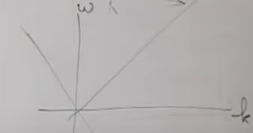
\includegraphics[width=\textwidth]{2-8-massless}
	\end{subfigure}
	\begin{subfigure}[t]{0.45\textwidth}
		\caption{Massive: non-linear dispersion relation. Different wavelengths propagate with different velocities, so wave disperses.}\label{fig:2-8-massive}
		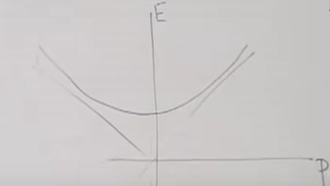
\includegraphics[width=\textwidth]{2-8-massive}
	\end{subfigure}
\end{figure}

For a particle with mass, $E=\sqrt{p^2 c^2 + m^2 c^4}$--Figure \ref{fig:2-8-massive}. Infinite wavelength still has non-zero $E$ (infinite wavelength means that the field is absolutely homogeneous). Whole field oscillates. Oscillations of a homogeneous field are what we call mass.

Mass is connected with the curvature of potential energy at the equilibrium point. If we shift system away it starts to oscillate, and $\omega \ne 0$ at $k=0$; in fact $\omega = m$. The only way this doesn't happen is if potential energy is flat. In Figure \ref{fig:mexican-hat}, we have a flat direction along dip, but not along radius. We therefore have two kinds of quanta:
\begin{itemize}
	\item massive--the Higgs boson;
	\item massless--the Goldstone boson. There is no massless Goldstone boson in nature, so something happened to it.
\end{itemize}

\begin{figure}[H]
	\begin{center}
		\caption[Mexican Hat potential]{Mexican Hat potential, with an unstable equilibrium at the origin.  The minimum is a circle centred on the origin: we can set a particle vibrating without expending any energy.}\label{fig:mexican-hat}
		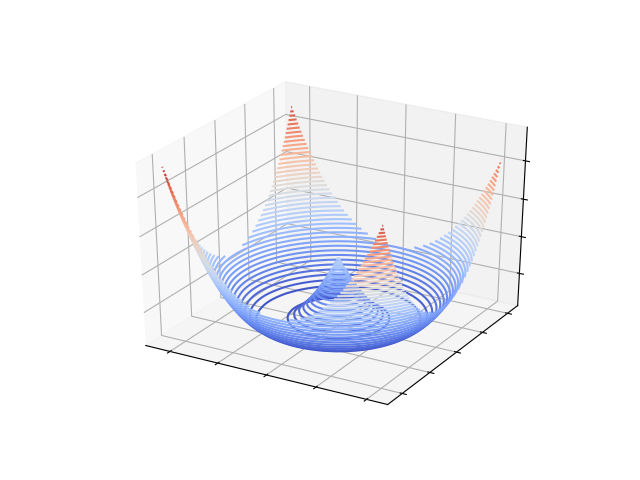
\includegraphics[width=0.6\textwidth]{mexican-hat}
	\end{center}
\end{figure}

''The Goldstone boson got eaten by the gauge boson, resulting in giving the Higgs boson a mass.''--this is the phenomenon which we want to do mathematically in this lecture.

There is a collection of particles in the standard model that cannot have mass unless there is spontaneous symmetry breaking. Are there any that don't require spontaneous symmetry breaking? Yes, \emph{they are the particles that we don't see in the laboratory.} The natural mass may be very large, up by the Planck mass, beyond the range of our accelerators. These may be the dark matter particles.

The first class that cannot get a mass without spontaneous symmetry breaking are the gauge bosons. We'll start with a field:

\begin{align*}
	\Phi =& \Phi_R + i \Phi_I \text{, or}\\
	=& \rho e^{i \alpha}\\
	\Phi^* =& \Phi_R - i \Phi_I \text{, or}\\
	=& \rho e^{-i \alpha}
\end{align*}

In Figure \ref{fig:mexican-hat}, $\alpha$ corresponds to angular motion (massless), $\rho$  to radial (massive).

\begin{align*}
	\mathcal{L} =& \partial \Phi^* \partial \Phi - V(\Phi^*\Phi)  \numberthis \label{eq:mexican:LagrangeRI}\\
	=& (\partial \rho)^2 + \rho^2 (\partial \alpha)^2 - V(\rho) \numberthis \label{eq:mexican:Lagrange}
\end{align*} 

If we take the simplest V, $\rho^2$
\begin{align*}
	\mathcal{L} = (\partial \Phi_R)^2 +  (\partial \Phi_I)^2 -(\Phi_R)^2  -(\Phi_I)^2
\end{align*}
which gives two uncoupled oscillations. This representation isn't so useful for Figure \ref{fig:mexican-hat}. In (\ref{eq:mexican:Lagrange}) we have two uncoupled oscillations. $V$ has a minimum at $f$. We let

\begin{align*}
	\rho = f + H \text{, the Higgs field}
\end{align*}

We will say that the low energy behaviour of $\rho$ is frozen at $f$, and (\ref{eq:mexican:Lagrange}) becomes:

\begin{align*}
	\mathcal{L} =& f^2(\partial \alpha)^2 \text{, at low energy.}\\
	=& (\partial \beta)^2 \text{, where $\beta = f \alpha$}
\end{align*}

$\beta$ is a massless field, the Goldstone boson. Goldstone bosons are massless particles which are the consequence of spontaneous symmetry breaking of a continuous symmetry.

\subsection{Local variation of gauge invariance--Goldstone bosons}

\begin{defn}[Scalar field]
	A scalar field is one which doesn't change when we rotate space.
\end{defn}

A complex number is a means of talking about pairs of numbers. Given two real fields I can assemble them into a single complex field. Don't confuse a complex scalar field with a vector field: we are dealing with different spaces.

The Lagrangian of (\ref{eq:mexican:LagrangeRI})  does not change when we rotate the complex plan in the fictitious field by an constant angle. This is a global symmetry.

We saw in Section \ref{section:gauge:invariance} that it is not a  symmetry to rotate by an angle that varies from point to point:
\begin{align*}
	\Phi^\prime (x) = e^{i\theta(x)} \Phi(x) \text{, this adds $\theta$ to $\alpha$}
\end{align*}

We saw that can fix this by introducing a vector potential $A_\mu$ and defining the covariant derivative $D$:
\begin{align*}
	A^\prime_\mu(x) =& A_\mu(x) + \partial_\mu \theta(x)\\
	\partial_\mu \Phi^\prime =& e^{i\theta} \big[\partial_\mu \Phi + i \partial_\mu \theta \,\Phi\big] \text{. The term containing $\partial \theta$  wrecks the symmetry}\\
	D_\mu \Phi \triangleq& \partial_\mu \Phi + i A_\mu \Phi\\
	D_\mu \Phi^* =& \partial_\mu \Phi^* - i A_\mu \Phi^* \text{. In Section \ref{section:gauge:invariance} we saw that:}\\
	D_\mu \Phi^\prime =& \partial_\mu \Phi^\prime + i A^\prime_\mu \Phi^\prime \\
	=& (D_\mu \Phi)^\prime \text{. The operators commute!}
\end{align*}

$\Phi$ is a charge carrying boson field, and $A_\mu$ is the electromagnetic potential: $F_{\mu\nu}=\partial_\mu A_\nu-\partial_\nu A_\mu$ is gauge invariant. The Lagrangian has the form $D\Phi^* D\Phi -V(\Phi^*\Phi) +F^2$. 

All gauge theories have a similar structure to this one.

\subsection{The Higgs phenomenon}

What happens when a potential such as Figure \ref{fig:mexican-hat} breaks the symmetry?

The $F$ is massless, as it contains only derivatives: it isn't changed by shifting in space. So we have two massless particles, the Goldstone boson and the photon. If photon had mass we have a term proportional to $A^2$. This isn't gauge invariant: $A^2 \rightarrow (A+\partial \theta)^2$. Gauge invariance prohibits mass

\begin{align*}
	\mathcal{L} =& D\Phi^* D\Phi -V(\Phi^*\Phi) +F^2\\
	=& \big( \Phi^* - i A \Phi^*\big) \big( \Phi + i A \Phi\big) -V(\Phi^*\Phi) +F^2
\end{align*}

Let us look at $\Phi = f$. Then the Lagrangian contains a term $f^2A^2$, which behaves like a mass $\sqrt{2}f$.

When we spontaneously break symmetry and consider field near $f$, photon behaves as if it had a mass.

The Goldstone boson disappears. The Goldstone boson is a slowly varying $\alpha$. We can make $\alpha$ vary by gauge transformation, which surely involves the Goldstone boson. But gauge transformation is a symmetry; it doesn't change energy and remains in the ground state. The Goldstone boson disappears, and the massless photon is replaced by a massive one. The Higgs boson now has a mass. That is the Higgs phenomenon.


Freeze radial variable.

\begin{align*}
	D \Phi = (\partial \alpha + iA)e^{i\alpha}f\\
	D \Phi^* = (\partial \alpha - iA)e^{-i\alpha}f
\end{align*}

We make a gauge transformation to get rid of $\alpha$: we subtract $\theta$. All that is left of the Lagrangian is $F^2+f^2A^2$. The angular degree of freedom disappears, Goldstone is gone, photon gets a mass.

This is also what happens in super-conductance. There are charge bosons, "Cooper pairs" of electrons. Charged boson field is shifted from origin, and gives rise to a broken symmetry.


\section{The Higgs field and fermions}

\subsection{Bosons}

The gauge bosons, Z and W, get their mass from the Higgs mechanism. Keep in mind that we aren't really talking about the photon, but ut will be useful to develop the maths as if we were.

There is a dynamics Maxwell's equations:
\begin{align*}
	F_{\mu\nu}=&\frac{\partial A_\mu}{\partial x^\nu}-\frac{\partial A_\nu}{\partial x^\mu}\\
	\mathcal{L} =& F_{\mu\nu} F^{\mu\nu} \text{, this has no energy from shift, so it is massless.}
\end{align*}

Now we add the Higgs field:
\begin{align*}
	\Phi =& \rho e^{i \alpha}\\
	D \Phi =& \partial \Phi + i A \Phi\\
	=& i \big( \partial \alpha + A \big) f e^{i \alpha} \text{, if $\rho$ frozen}\\
	\mathcal{L} =& f^2 \big(\partial \alpha + A \big)^2 \text{, now make a gauge transformation}\\
	=& f^2 {A^\prime}^2
\end{align*}

If we shift $A^\prime$ everywhere, we'd get some energy from $f^2 {A^\prime}^2$. \emph{We have introduced mass!} Vacuum shifted to some new spontaneously broken, and excitations of field in that vacuum have a mass. $\alpha$ has disappeared.

There is still the thing that we froze in an approximation. What if we hit it hard enough to set it oscillating in radial direction? These are the Higgs bosons.
 
\subsection{Fermions}

Where do they get their mass?

We go back to weak interactions.

Reflection symmetry is not a good symmetry of elementary particles (1950s). This is a symmetry of \gls{gls:QM} and QCD, but it is not a symmetry of the weak interaction (mirror image of a weak interaction is not another possible process!). 

\begin{figure}[H]
	\caption{The electron is always left handed in n weak interactions}
	\begin{subfigure}[t]{0.4\textwidth}
		\caption{Beta decay of a neutron}\label{fig:2-9-beta-decay-neutron}
		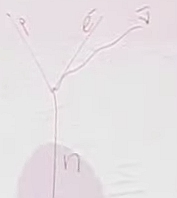
\includegraphics[width=0.8\textwidth]{2-9-beta-decay-neutron}
	\end{subfigure}
	\begin{subfigure}[t]{0.4\textwidth}
		\caption{W boson converting left handed electron to neutrino}\label{fig:2-9-W-boson}
		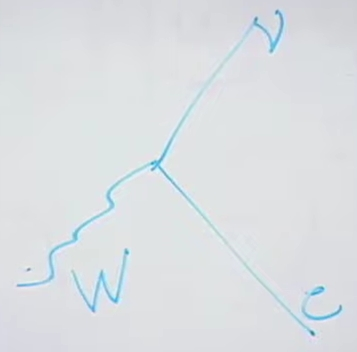
\includegraphics[width=0.8\textwidth]{2-9-W-boson}
	\end{subfigure}
\end{figure}

Is there a notion of handedness? Yes, we have spin and direction of motion. Either the electron rotates with direction of motion (right handed screw) or left handed. You might think that Figure \ref{fig:2-9-beta-decay-neutron} could make right-handed or left-handed neutrons, but the electrons are always left handed. Moreover in scattering by a W-boson, it is only the left handed electron that interacts with a W-boson--e.g. Figure \ref{fig:2-9-W-boson}. It is an experimental fact that the left-handed electron scatters, and the right handed one doesn't. Similarly it is always the left-handed neutrino that interacts: it is \emph{questionable} whether there are right handed neutrinos.

There is something asymmetric about weak interactions: it is as if left-handed particles carried "charge" associated with boson, but right don't.

Let's go back to the Dirac equation. The Dirac Field, $\Psi$, is a four component object: particles can have spin along either direction, up or down, and positive or negative energy.

\begin{align*}
	i \big(\frac{\partial \Psi}{\partial t} + \alpha_i \frac{\partial \Psi}{\partial 	x^i}\big) =&0
\end{align*}
 This would be Dirac equation if electron massless, because equation only involves derivatives of the field. There is no restoring force, no tendency to oscillate.
 
 \begin{align*}
 	i \big(\frac{\partial \Psi}{\partial t} + \alpha_i \frac{\partial \Psi}{\partial 	x^i}\big) =&m \beta \Psi \text{, Dirac equation with mass.}
 \end{align*}
 
 The electron could be moving along with a momentum so there is a gradient, $\frac{\partial \Psi}{\partial x_i}$. Spin can be along or opposite to direction of motion. 
 
 \begin{align*}
 	i \big(\frac{\partial \Psi_R}{\partial t} + \alpha_i \frac{\partial \Psi_R}{\partial 	x^i}\big) =& m \Psi_L \text{, since $\beta$ interchanges R and L}\\
 	i \big(\frac{\partial \Psi_L}{\partial t} - \alpha_i \frac{\partial \Psi_L}{\partial 	x^i}\big) =& m \Psi_R \text{, mass couples L and R}
 \end{align*}
 
 Let us suppose that only left-handed particle has a charge (True for weak, not for electro-magnetic). Then we can't have these equations because of charge conservation. Another way to look at is the gauge transformation $e^{i\theta}$. Charge conservation would forbid a mass for the electron if only left had charge.
 
 Meanwhile back in the real world this isn't true.
 
 Suppose there were only a left handed electron. If it has mass we could slow it down, bring it to rest, then send it back; handedness would have changed although spin hadn't. What if no mass? Then we can't do this.
 
 How might electrons get a mass in this fake world where only left have electric charge? Imagine there is a Boson field, $\Phi$, whose quanta have positive charge.
 
 Under $U(a)$:
 \begin{align*}
 	\Psi_L \rightarrow& e^{i\theta} \Psi_L \text{, because charged}\\
 	\Psi_R \rightarrow& \Psi_R \text{, because not charged}\\
 	\Phi \rightarrow& e^{i\theta} \Phi \text{, because charged}
 \end{align*}
 Clearly Dirac equation is not invariant under $U(a)$. We will rewrite to be invariant:
 
 \begin{align*}
	 i \big(\frac{\partial \Psi_R}{\partial t} + \alpha_i \frac{\partial \Psi_R}{\partial 	x^i}\big) =& g \Phi^* \Psi_L \numberthis \label{eq:mod:Dirac:R}\\
	 i \big(\frac{\partial \Psi_L}{\partial t} - \alpha_i \frac{\partial \Psi_L}{\partial 	x^i}\big) =& g \Psi_R \Phi \numberthis \label{eq:mod:Dirac:L}
 \end{align*}
 
 Figure \ref{fig:modified:Dirac} shows how to interpret these equations in terms of Feynman diagrams. Left and right change into each other, and the cost of emitting charged particles, with coupling constant $g$, the \emph{Yukawa coupling}.
 \begin{figure}[H]
 	\caption{Interpretation of modified Dirac equation}\label{fig:modified:Dirac}
 	\begin{subfigure}[t]{0.3\textwidth}
 		\caption{RH electron $\rightarrow$ LH + $\bar{\Phi}$--(\ref{eq:mod:Dirac:R})}
 		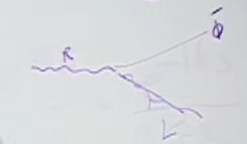
\includegraphics[width=\textwidth]{2-9-RH}
 	\end{subfigure}
  	\begin{subfigure}[t]{0.3\textwidth}
  		\caption{LH electron $\rightarrow$ RH + $\Phi$--(\ref{eq:mod:Dirac:L})}
	 	\includegraphics[width=\textwidth]{2-9-LH}
	 \end{subfigure}
   	\begin{subfigure}[t]{0.3\textwidth}
 	\caption{LH electron $\rightarrow$ RH + Higgs--(\ref{eq:fermion:Higgs})}\label{fig:2-9-Higgs-boson}
 	\includegraphics[width=\textwidth]{2-9-Higgs-boson}
 \end{subfigure}
 \end{figure}

What if $\Phi$ is a magical Higgs field, $\Phi=\rho e^{i\alpha}$? It has a spontaneous symmetry breaking $\Phi=f$ ($\alpha$ got eaten). (\ref{eq:mod:Dirac:R}) and (\ref{eq:mod:Dirac:L}) become:

 \begin{align*}
i \big(\frac{\partial \Psi_R}{\partial t} + \alpha_i \frac{\partial \Psi_R}{\partial 	x^i}\big) =& g f \Psi_L \\
i \big(\frac{\partial \Psi_L}{\partial t} - \alpha_i \frac{\partial \Psi_L}{\partial 	x^i}\big) =& g f \Psi_R  
\end{align*}

We use the mass of Z and W to determine $f$, so we can figure out $g$ from $m$. Since there are different masses for Fermions, there are multiple Yukawa couplings.

The Higgs particle is the fluctuation away from the frozen value. We should really write:
 \begin{align*}
i \big(\frac{\partial \Psi_R}{\partial t} + \alpha_i \frac{\partial \Psi_R}{\partial 	x^i}\big) =& g (f+H) \Psi_L  \numberthis \label{eq:fermion:Higgs}\\
i \big(\frac{\partial \Psi_L}{\partial t} - \alpha_i \frac{\partial \Psi_L}{\partial 	x^i}\big) =& g (f+H) \Psi_R  
\end{align*}

In (\ref{eq:fermion:Higgs}) and Figure \ref{fig:2-9-Higgs-boson} we see that RH can turn into LH + Higgs. When Higgs is found\footnote{This lecture predates the discovery at LHC.} we want to verify the relative rates of different Higgs interactions. 

None of the particles in the Standard Model would have mass if it were not for the Higgs Field. Gauge Bosons normally don't have mass: the only way to give them mass is via spontaneous symmetry breaking, and this mass is proportional to $f$. The Fermions, because all their interactions are left handed, so they need $f$ to acquire mass (Positron is right handed, BTW).

Left handed neutrino, right handed anti-neutrino. Ettore Majorana particle.

All particles of Standard Model trace their back to $f$; if $f$ were zero, they'd be massless. Why? Maybe we haven't found them because $f$ is around 250GeV, and that is the limit of what our current accelerators will do.

Imagine that a particle existed where L and R both had charge. Then there would be no limit on mass. Some people think that the limit on mass is much greater than $f$. Dark Energy?
Neutrinos can mix with anti-neutrinos and produce a massive Majorana particle which is its own antiparticle.

\section{Renormalization and the running of coupling constants}

\subsection{Lagrangian for Dirac Equation}

We want to derive the Dirac equation from a variational principle.
 \begin{align*}
	i \big(\frac{\partial \Psi}{\partial t} + \alpha_i \frac{\partial \Psi}{\partial 	x^i}\big) -m \beta \Psi =&0 \text{,  Dirac equation}
\end{align*}

\begin{align*}
	\mathcal{L}=&\Psi^\dagger i \big(\frac{\partial \Psi}{\partial t} + \alpha_i \frac{\partial \Psi}{\partial 	x^i} -m \beta \Psi\big)\text{. If we write}\\
	\bar{\Psi} \triangleq&\Psi^\dagger \beta  \\
	\Psi^\dagger  =& \bar{\Psi} \beta \text{, since $\beta^2=1$}\\
	\mathcal{L} =& \bar{\Psi}\beta \partial_t + \bar{\Psi}\beta \alpha_i \partial \Psi +m \bar{\Psi}  \Psi\\
	=& \bar{\Psi}\gamma_0 \partial_t + \bar{\Psi}\gamma_i \partial_i \Psi +m \bar{\Psi}  \Psi\\
	=& \bar{\Psi}\big(\gamma^\mu \partial_\mu +m  \big) \Psi \text{. The term $\gamma^\mu \partial_\mu$ does not couple LH \& RH} \numberthis \label{eq:dirac:lagrange}
\end{align*}
There is a fifth Dirac matrix:
\begin{align*}
	\gamma_5 \triangleq & \gamma_0 \gamma_1 \gamma_2 \gamma_3 \text{, \emph{not} $\gamma_4$!}\\
	\gamma_5^2 =&1
\end{align*}

Eigenvalues $\pm 1$--correspond to LH and RH.

\begin{defn}[chirality]
	$\gamma_5^2$ is called chirality.
\end{defn}

In (\ref{eq:dirac:lagrange}), we noted that $\gamma^\mu \partial_\mu$  does not couple LH and RH, i.e. the eigenvectors of $\gamma_5^2$ corresponding to $\pm 1$. But

\begin{thm}[The mass term in  (\ref{eq:dirac:lagrange}) mixes up left and right]
	\begin{align*}
		\bar{\Psi}\Psi =& \Psi^\dagger_L \Psi_R + \Psi^\dagger_R \Psi_L \numberthis \label{eq:LR}
	\end{align*}
\end{thm}
\begin{proof}
	TBP
\end{proof}

so the mass term in  (\ref{eq:dirac:lagrange}) mixes up left and right. A Dirac mass is a term in the Lagrangian which causes left and right fermions to flip. A massless Fermion has a definite chirality, but a massive one flips.

\subsection{The W boson and mass scale for Higgs boson}

We talked about weak interactions, in particular the emission and absorption of W and Z bosons. For some reason the W boson is emitted only by left handed particles (not true for photons, more complicated for Z, which has asymmetric couplings to LH and RH). So for $SU(2)$ the left handed particles are "charged". The term (\ref{eq:LR}) is not legal in a Lagrangian if it would take charged to uncharged.

So how do we get a mass for Fermions? Higgs also plays role as charged object for $SU(2)$ for weak interactions. In fact it is a doublet, like electron/neutrino. Higgs transforms under $SU(2)$. We need to multiply term in (\ref{eq:LR}) by Higgs field; the Higgs either has no charge or the opposite charge to particle. Figure \ref{fig:2-10-Higgs-emitted} and (\ref{eq:higgs:emitted}) illustrate the process of Higgs, $\Phi$, carrying off the weak charge.

\begin{align*}
	g_y \bar{\Psi}\Psi =& g_y \Psi^\dagger_L \Phi \Psi_R + g_y \Psi^\dagger_R \Psi_L \Phi^\dagger \text{, where $g_y$ is the Yukawa coupling} \numberthis \label{eq:higgs:emitted}
\end{align*}

\begin{figure}[H]
	\caption[Higgs interacting with Fermions]{Higgs interacting with Fermions: two forms of the same diagram}
	\begin{subfigure}[t]{0.45\textwidth}
		\caption{Higgs carries off weak charge}\label{fig:2-10-Higgs-emitted}
		\feynmandiagram[vertical=i2 to i1]{
			i1[particle=L] -- [fermion] a -- [fermion] i2[particle=R],
			a--[charged scalar,edge label=weak charge] b[particle=$\Phi$]
		};
	\end{subfigure}
	\begin{subfigure}[t]{0.45\textwidth}
		\caption{Higgs decaying into electron + positron}\label{fig:2-10-Higgs-decaying}
		\feynmandiagram[vertical=o1 to i1]{
			i1[particle=$\Phi$]--[charged scalar] a --[fermion] o1 [particle=$e^-$],
			a --[anti fermion] o2 [particle=$e^+$]
		};
	\end{subfigure}
\end{figure}

That would be the end of the story, except that Nature has chosen a Mexican Hat potential for the Higgs field, so we have a fluctuation, $\Phi=f+H$.

\begin{align*}
g_y \bar{\Psi}\Psi =& g_y f \big(\Psi^\dagger_L  \Psi_R +  \Psi^\dagger_R \Psi_L  \big) + g_y\underbrace{ H \big(\Psi^\dagger_L  \Psi_R +  \Psi^\dagger_R \Psi_L  \big)}_\text{Emit electron and re-emit it plus Higgs}
\end{align*}

The same $f$ is used for the Z and W bosons ($\approxeq200GeV$), so we can use observed masses to determine $g_y$ (different for each type of particle). Figure \ref{fig:2-10-Higgs-emitted} can be redrawn as a single Higgs decaying, Figure \ref{fig:2-10-Higgs-decaying}, so, once we can find a Higgs in the laboratory, we should be able to predict decay rates.

At the time of the lecture the Higgs had not been found: however there seems to be no way to make the mathematical theory consistent without the Higgs. The theory does make verifiable productions about the Z and W bosons.


\subsection{Dynamics of the Higgs boson}

This is all contained in Mexican Hat potential--Figure \ref{fig:2-10-MexicanHat}
\begin{figure}[H]
	\caption{Mexican Hat Potential for Higgs}\label{fig:2-10-MexicanHat}
	\includegraphics[width=0.8\textwidth]{2-10-MexicanHat}
\end{figure}
One such function is:
\begin{align*}
	V =& -\frac{\mu^2}{2} \phi^2 + \frac{\lambda}{4} \phi^4 \text{. The first term would represent mass if it were positive}
\end{align*}

The "imaginary mass" isn't a problem; having the origin be unstable is odd, so we introduce the quartic coupling constant $\lambda$ to prevent $\phi$ falling indefinitely. It appears\footnote{Indirect evidence from weak interactions} that $\lambda$ is small, but not absurdly small, around 0.01 ($\mu$ has dimensions of mass).

We want to find $f$, the $\phi$ which gives the minimum of $V$.
\begin{align*}
	\frac{d V}{d \phi} =& -\mu^2 \phi + \lambda \phi^3\\
	=& \phi \big(\lambda \phi^2 - \mu^2\big)\\
	=& 0 \text{, at a minimum. Since $\phi=0$ is unstable}\\
	f =& \frac{\mu}{\sqrt{\lambda}}
\end{align*}

$f$ is mass of Z or W Bosons, and it comes into mass of Fermion. It controls the masses of all the particles we know about: why are they all controlled by the same phenomenon? Why are there no particles whose mass doesn't involve spontaneous symmetry breaking? E.g. we can imagine a particle whose left and right variants both have weak charge: we wouldn't need $\Phi$. Or particles without weak interactions?

The general thinking (i.e. a widespread \emph{belief}) is that the mass scale is enormous, much higher that those of the known particles, and that the only small mass parameter is $f$; only those particles that are this light have been detected. But why is $f$ so small? (compared with what?) 

The Planck Mass and Unification Mass are about 15 orders of magnitude larger than $f$.

Bose condensates. Helium is not normally considered an elementary particle, but, at some scale it can be treated as one. There is a Helium field, that is normally zero. Spontaneous symmetry breaking can happen and create superfluidity.

If $He$ charged it can behave like a Higgs, and give mass to the photon. We have Cooper pairs of electrons, which can condense.

\subsection{What is the normal mass scale for elementary particle physics?}

We start with Lagrangian, which includes a bunch of parameters--such as mass and charges. But when we measure, we get numbers that are a product of a whole lot of interactions between high and low frequency modes, which renormalize values of parameters.

One example is electric charge. The normally observed charge is determined by Coulomb law for things at a large distance: $V=\frac{e^2}{R}$. This is asymptotically true for large $R$.

If you do this in a material you will get a different value; you will get a slightly reduced value (except in a vacuum). What if we put a charge into a conductor? Field causes motion of charges until charges flow to boundary--Figure \ref{fig:2-10-charged-conductor}. Figure \ref{fig:2-10-neg-charged-conductor} shows the same thing with a negative charge. We find that there is no attraction: experimental charge is not what we put in.

\begin{figure}[H]
	\caption{Charged conductor}
	\begin{subfigure}[t]{0.45\textwidth}
		\caption{Charged flows out to distant boundary, and get surrounded by opposite charge.}\label{fig:2-10-charged-conductor}
		\includegraphics[width=\textwidth]{2-10-charged-conductor}
	\end{subfigure}
	\begin{subfigure}[t]{0.45\textwidth}
		\caption{Negative charge}\label{fig:2-10-neg-charged-conductor}
		\includegraphics[width=\textwidth]{2-10-neg-charged-conductor}
	\end{subfigure}
\end{figure}

Let's move the charges together, assuming charges are smaller than the clouds. Make them be closer than cloud, then we do feel coulomb force. We could say that charge is a function of distance, and $V=\frac{e(R)^2}{R}$, where $e(R)$ is the \emph{running charge}.

Now consider a dielectric. Electrons are bound to atoms, but there is some movement allowed. There will be some screening; diminished attraction from Coulomb law. We still have $e(R)$, but it doesn't go all the way to zero at infinity.

This is exactly what happens in \gls{gls:QFT}. Vacuum is basically a dielectric. Charge that is felt at a large distance is not the bare electric charge in Lagrangian. Separation between members of a virtual pair depends on virtual energy. As you bring charged particles closer, screening from low energy virtual pairs will not be there--Figure \ref{fig:2-10-effective-charge}

\begin{figure}[H]
	\caption{Running charges}
	\begin{subfigure}[t]{0.45\textwidth}
		\caption{EM Running charge increasing logarithmically with $\frac{1}{R}$}\label{fig:2-10-effective-charge}
		\includegraphics[width=\textwidth]{2-10-effective-charge}
	\end{subfigure}
	\begin{subfigure}[t]{0.45\textwidth}
		\caption{Weak, Strong and EM Running charge}\label{fig:2-10-effective-charge-esw}
		\includegraphics[width=\textwidth]{2-10-effective-charge-esw}
	\end{subfigure}
\end{figure}

If you scatter at low energy, charge, and hence scattering, is reduced. "True" charge is what we see at the smallest distances (except we don't know what happens at the Planck Length).

Renormalization: how do we have to change the charge at smaller and smaller distances to keep the physics matching experiment?

Strong Interactions are more complicated. Force law between quarks foes not behave like $\frac{e^2}{R}$. We get the tube-like structures of Figure \ref{fig:QCD:QED}. Energy grows linearly, $\propto R$. We can make $e(R) \propto R$ and salvage Coulomb's law.

Figure \ref{fig:2-10-effective-charge-esw} shows the variation of the weak, strong, and EM charges. Notice that they come together at a common point. It looks as if they are unified at some high energy. In the Supersymmetric version they unify at $10^{16}GeV$ (curves vary slowly). This would suggest that this is fundamental length. If you plot gravitational forces, they don't cross at the same point, but within a couple of decades of length.

\subsection{Gravitational forces}

$\frac{1}{R^3}$ at small distances.

\begin{align*}
	F =& \frac{mm}{R^2}G \text{, non-relativistic}\\
	=& \frac{E E}{c^4 R^2}G \text{,                                              relativistic}
\end{align*}

Let's bring them close (Compton Length), so $P\approxeq\frac{\hslash}{R}$


\begin{align*}
	E =& Pc\\
	=& \frac{\hslash c}{R}\\
	F =& \frac{\hslash^2 c^2}{R^4 c^2}G
\end{align*}

At what scale is gravitational force comparable to EM?

\begin{align*}
	\frac{\hslash^2 c^2}{R^4 c^2}G =& \frac{e^2}{R^2} \text{, new set $e=1$}\\
	\frac{\hslash^2 c^2}{R^4 c^2}G =& \frac{1}{R^2} \\
	R =&\frac{\hslash \sqrt{g}}{c}	\text{, check!}
\end{align*}
This is the Planck length.


% glossary: may need command makeglossaries.exe particles2
\printglossaries

\bibliographystyle{unsrt}
\addcontentsline{toc}{section}{Bibliography}
\raggedright
\bibliography{tm}


\end{document}
